%!TEX root = ../report.tex

\begin{document}
    \chapter{Experiments and Results}
    %In this chapter, we will discuss about the experiments conducted for out-of-distribution (OOD) detection on RandLA-Net using uncertainty techniques such as deep ensembles and flipout.
    %These experiments were conducted on Semantic3D dataset as training in-distribution (ID) dataset and two datasets particularly S3DIS and Toronto3D are used as OOD datasets. 
    %The detailed description about datasets can be found in Chapter \textcolor{red}{cite here}, about RandLA-Net in Section \textcolor{red}{cite here}, and about deep ensembles and flipout in Section \textcolor{red}{cite here}
    %The list of experiments conducted to acheive OOD detection are as follows:
    This chapter discusses the experiments conducted for Out-Of-Distribution (OOD) detection on RandLA-Net using quantified uncertainty from Deep Ensembles and Flipout.
    In a detailed discussion about RandLA-Net, Deep Ensembles and Flipout can be found in Chapter~[\$]. In this chapter, we first discuss the training results of RandLA-Net using deep ensembles and flipout on Semantic3D as an In-Distribution (ID) dataset.
    Furthermore, we compare the Maximum Softmax Probability (MSP) as in \cite{hendrycks2016baseline_MSP} and entropy values for the proposed OOD benchmark datasets Semantic3D vs S3DIS and Semantic3D vs Semantic3D w/o colour.
    Finally, we visualize and evaluate the performance of OOD detection using the AUROC score.

%%%%%%%%%%%%%%%%%%%%%%%%%%%%%%%%%%%%%%%%%%%%%%%%%%%%%%%%%%%%%%%%%%%%%%%%%%%%%%%
    %%%%%% Deep ensmebles performance %%%%%%
    \section{Deep Ensembles-Semantic3D}
    \label{sec:deepensemble_train}
    In this experiment, we trained 20 models of RandLA-Net over the Semantic3D dataset using random initializations with the experimental setup described in Section~[\$].
    The predictions from these 20 individual models are then averaged to compute the final predictions.
    The evaluation results of the Deep Ensembles are described in Table~\ref{tab:ensemble_eval} using meanIoU, per-class IoU and accuracy.
    The predictions from the Deep Ensembles are depicted in Figure~\ref{fig:deepensemble_vis_sem3d} and Figure~\ref{fig:deepensemble_improv}.
    \begin{table}[h!]
        \resizebox{\textwidth}{!}{%
        \begin{tabular}{c|c|cccccccc|c}
        %\textbf{\#Ensembles} & \textbf{MeanIOU} & \textbf{Accuracy} & \textbf{Manmadeterrain} & \textbf{Naturalterrain} & \textbf{Highvegetation} & \textbf{Lowvegetation} & \textbf{Buildings} & \textbf{Hardscapes} & \textbf{Scanningartifacts} & \textbf{Cars} \\ \hline
        & & \multicolumn{7}{c}{\textbf{IoU per class}} & \\ \hline
        \textbf{Ensemble size} & \textbf{meanIoU} & \textbf{C1} & \textbf{C2} & \textbf{C3} & \textbf{C4} & \textbf{C5} & \textbf{C6} & \textbf{C7} & \textbf{C8} & \textbf{Accuracy} \\ \hline
        1& 68.19& 94.55& 81.19& 84.67& 29.43& 81.37& 18.85& 64.74& 90.74& 88.78 \\
        5& 69.51& 94.73& 81.92& 84.42& 28.05& \textbf{86.41}& 28.50& 61.03& 91.03& 90.04 \\
        10& 69.97& 95.25& 83.73& 86.63& 30.36& 84.13& 18.60& \textbf{66.01}& 92.61& 89.94 \\
        15& 70.32& 95.27& 83.54& \textbf{88.22}& \textbf{32.19}& 84.82& 26.17& 61.67& 90.75& \textbf{90.57} \\
        20& \textbf{70.80}& \textbf{95.55}& \textbf{84.11}& 86.65& 29.60& 85.41& \textbf{29.58}& 62.47& \textbf{93.06}& 90.56 \\
        \end{tabular}%
        }
        \caption{Illustration of performance of RandLA-Net on Semantic3D over number of ensembles. meanIOU and IOU per-class and overall accuracy are represented here.
        C1 to C8 are the classes of Semantic3D which are Manmadeterrain, Naturalterrain, Highvegetation, Lowvegetation, Buildings, Hardscapes, Scanningartifacts, and Cars.}
        \label{tab:ensemble_eval}
    \end{table} 

    \begin{figure*}[h!]
        \begin{tabular}{ccc}
            RGB & Ground Truth & Prediction-Deep Ensembles \\
            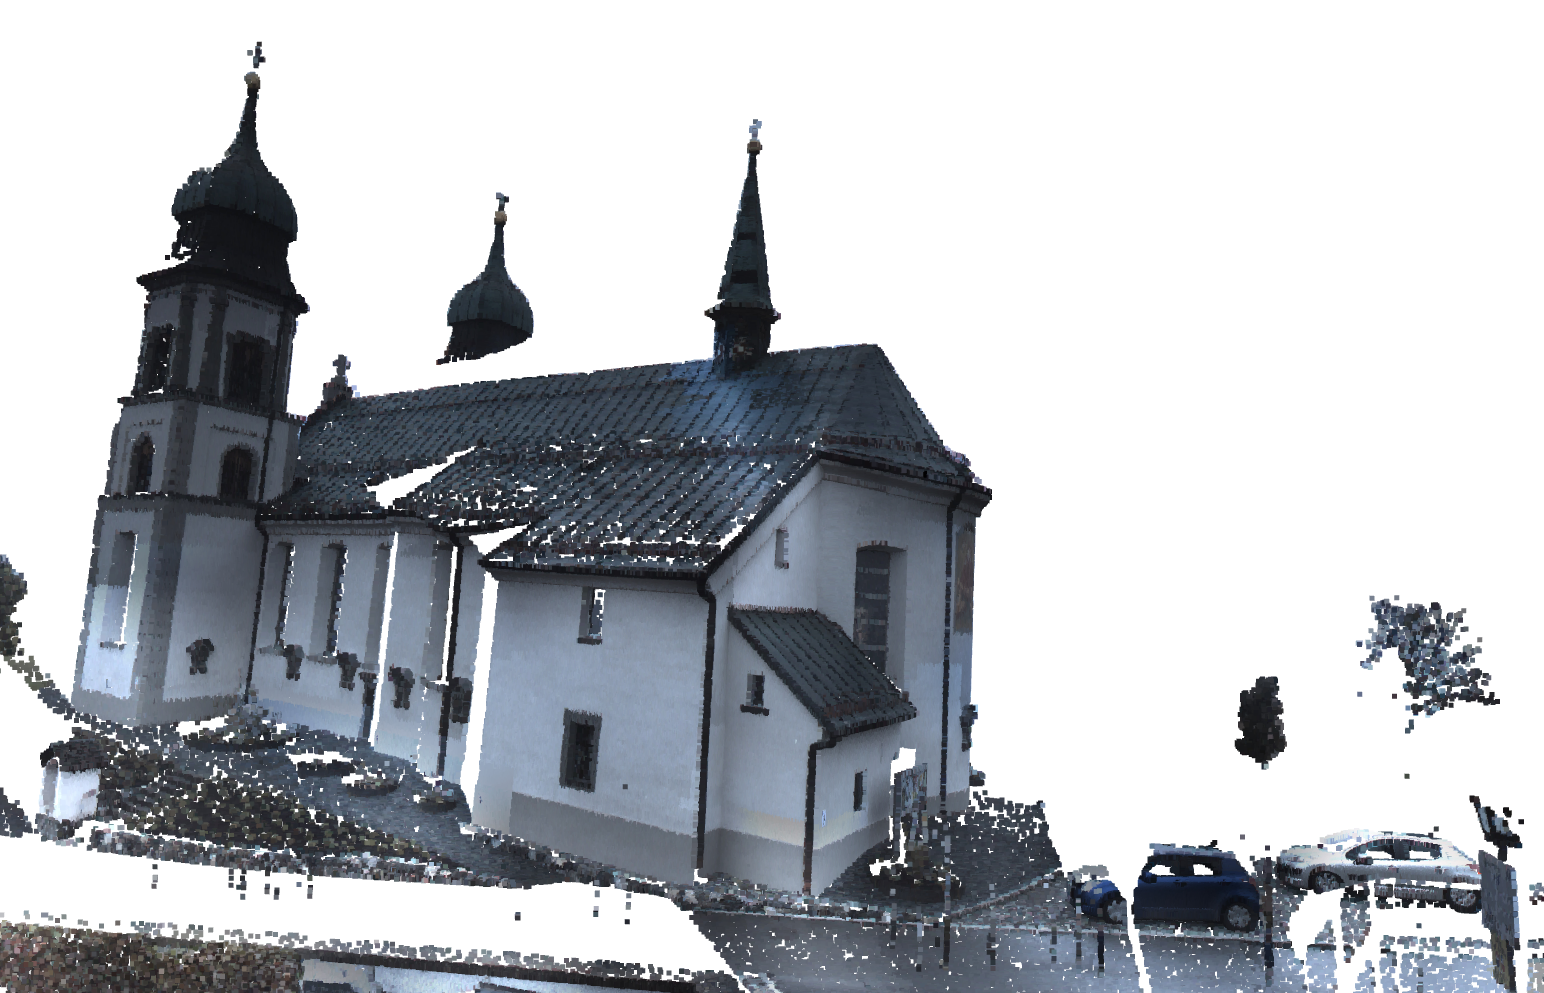
\includegraphics[width=0.33\textwidth, height=0.18\textheight]{images/seg_output/sem3d_seg_output/1_RGB.png} &
            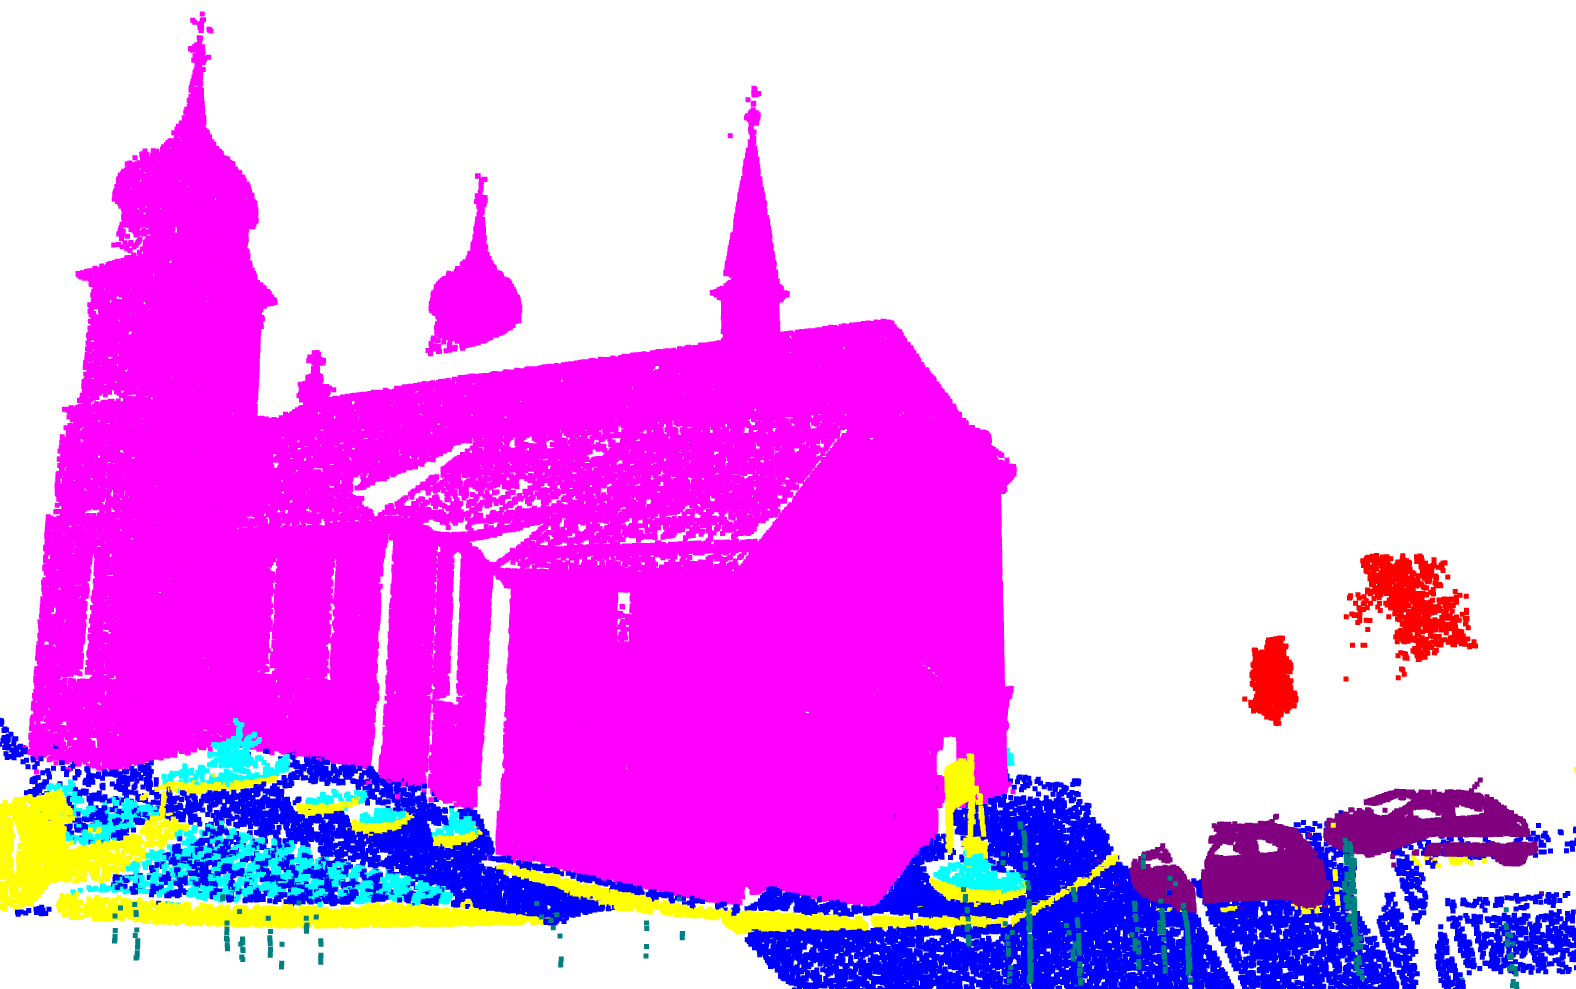
\includegraphics[width=0.33\textwidth, height=0.18\textheight]{images/seg_output/sem3d_seg_output/1_GT.png}& 
            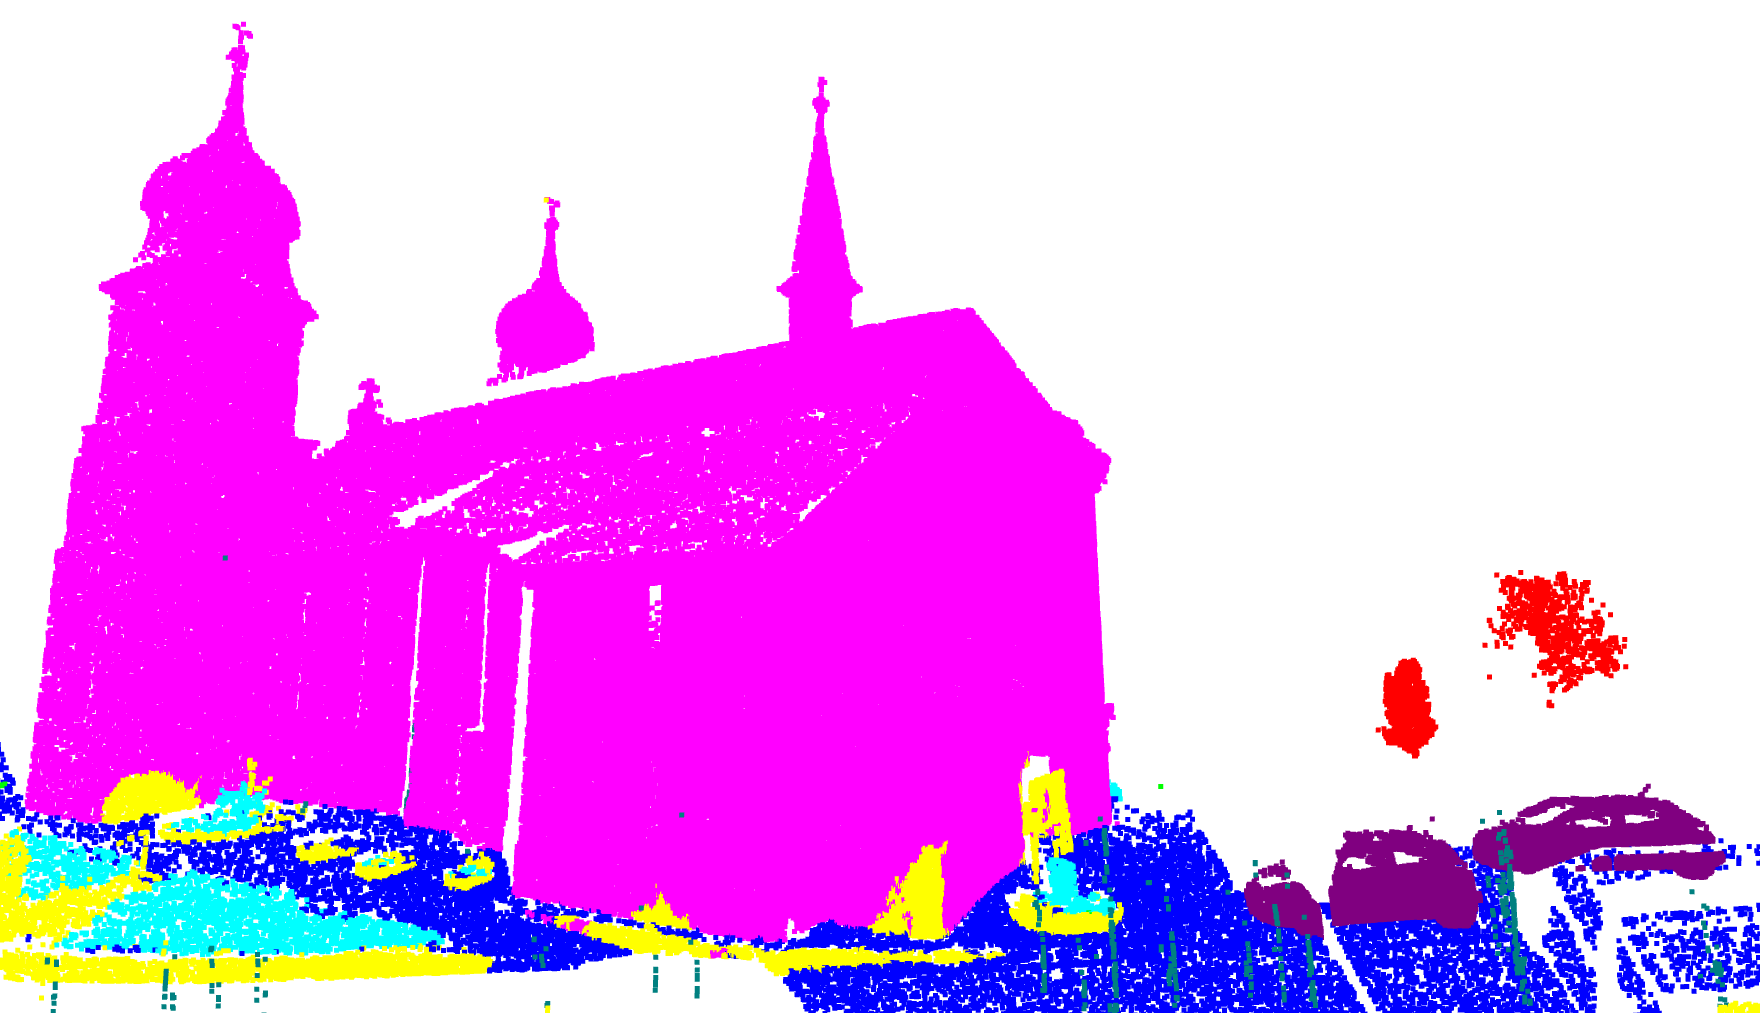
\includegraphics[width=0.33\textwidth, height=0.18\textheight]{images/seg_output/sem3d_seg_output/1_Pred.png}\\

            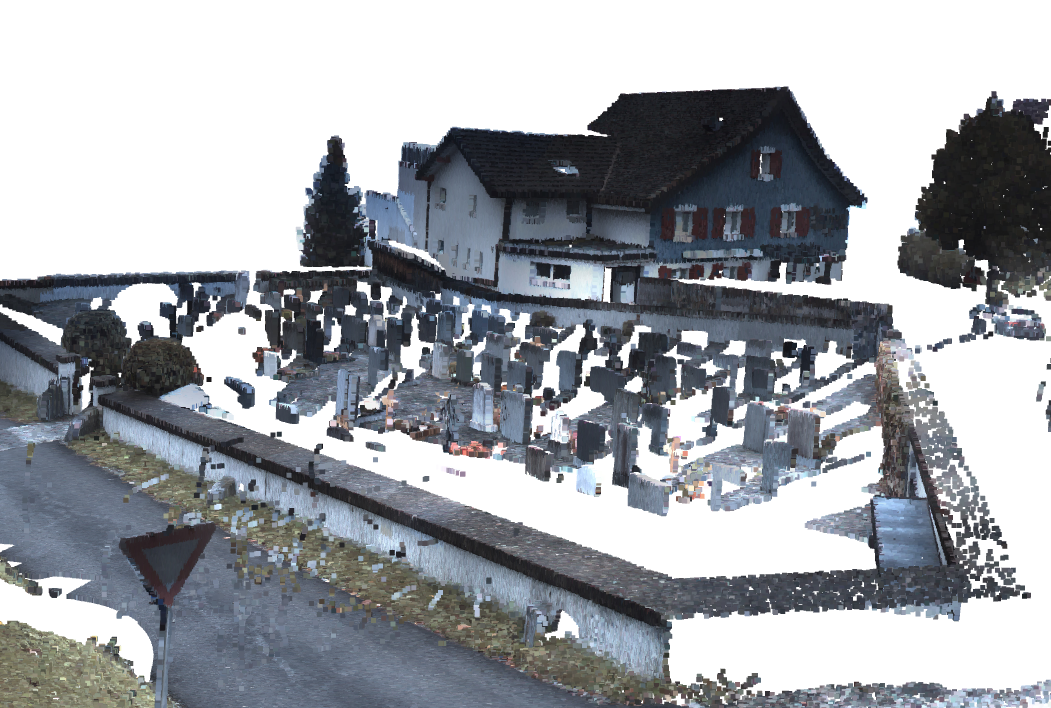
\includegraphics[width=0.33\textwidth, height=0.18\textheight]{images/seg_output/sem3d_seg_output/2_RGB.png} &
            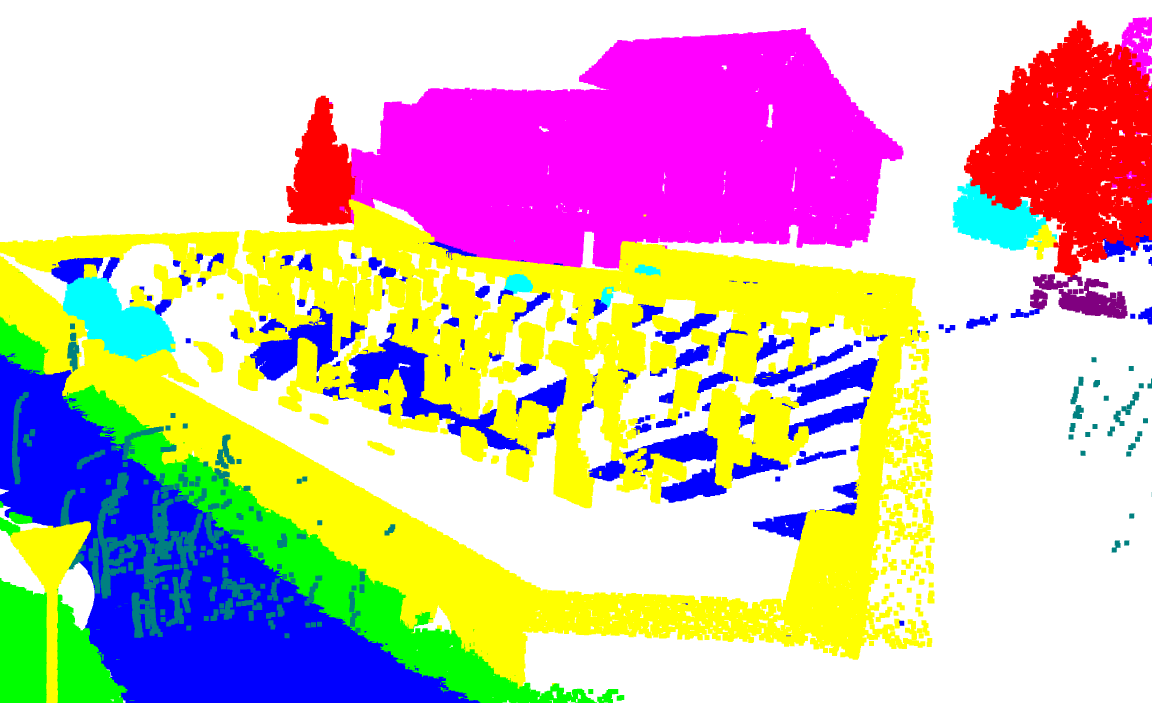
\includegraphics[width=0.33\textwidth, height=0.18\textheight]{images/seg_output/sem3d_seg_output/2_GT.png}& 
            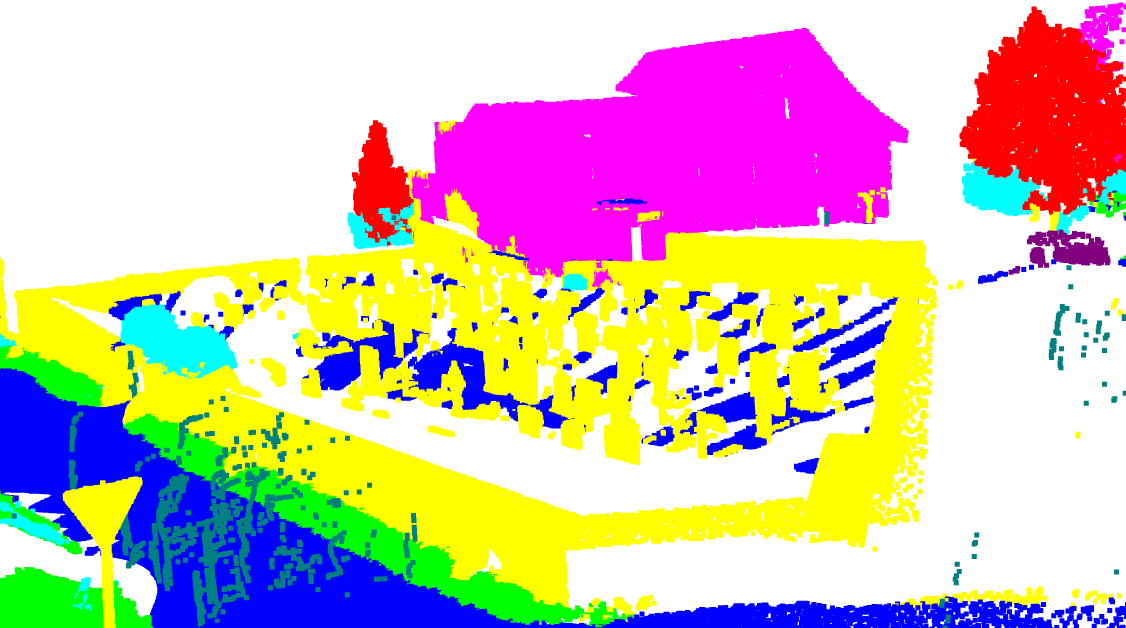
\includegraphics[width=0.33\textwidth, height=0.18\textheight]{images/seg_output/sem3d_seg_output/2_Pred.png}\\

            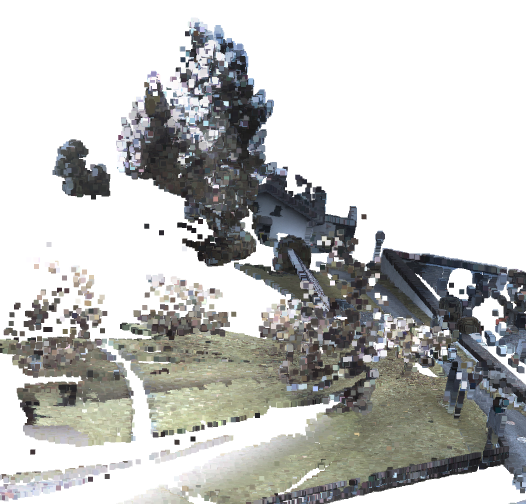
\includegraphics[width=0.33\textwidth, height=0.18\textheight]{images/seg_output/sem3d_seg_output/3_RGB.png} &
            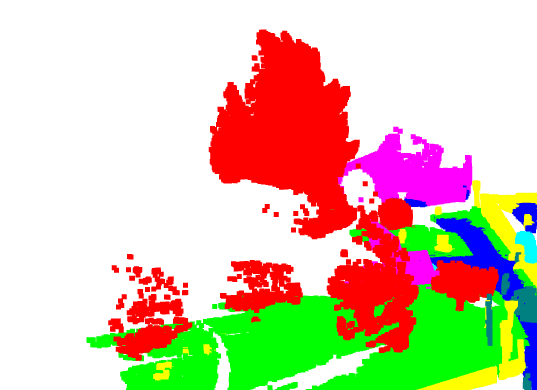
\includegraphics[width=0.33\textwidth, height=0.18\textheight]{images/seg_output/sem3d_seg_output/3_GT.png}& 
            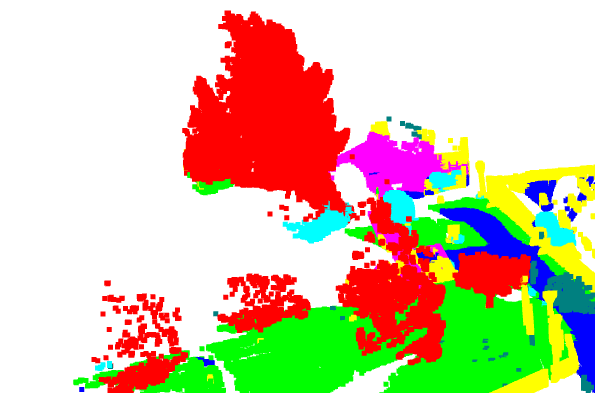
\includegraphics[width=0.33\textwidth, height=0.18\textheight]{images/seg_output/sem3d_seg_output/3_Pred.png}\\
        \end{tabular}
        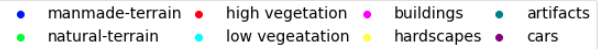
\includegraphics[scale=0.65]{images/legend.png}
        \caption{Output predictions of the RandLA-Net over the Semantic3D dataset (13 ensemble size) \textcolor{red}{Legend spelling mistake}.}
        \label{fig:deepensemble_vis_sem3d}
    \end{figure*}

    % %%%%%% Segmentation output here %%%%%%
    
    % %%%%%% Ensembles output here %%%%%%
    \begin{figure*}[h!]
        \begin{tabular}{cccc}
            1 & 5 & 10 \\
            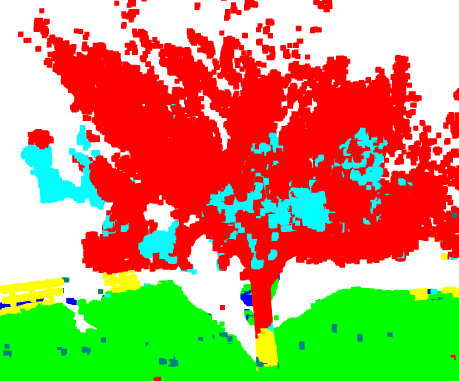
\includegraphics[width=0.30\textwidth, height=0.15\textheight]{images/seg_output/deep_ensembles/1_1.png} &
            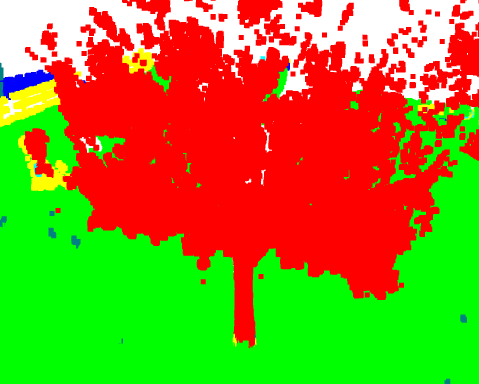
\includegraphics[width=0.30\textwidth, height=0.15\textheight]{images/seg_output/deep_ensembles/1_5.png}& 
            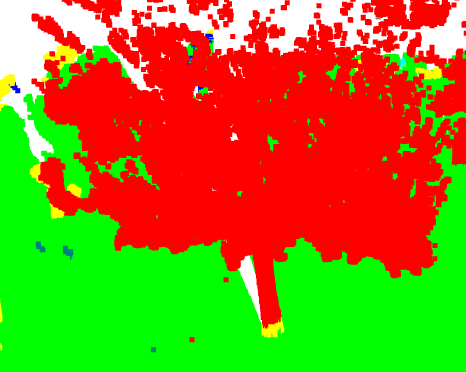
\includegraphics[width=0.30\textwidth, height=0.15\textheight]{images/seg_output/deep_ensembles/1_10.png}\\

            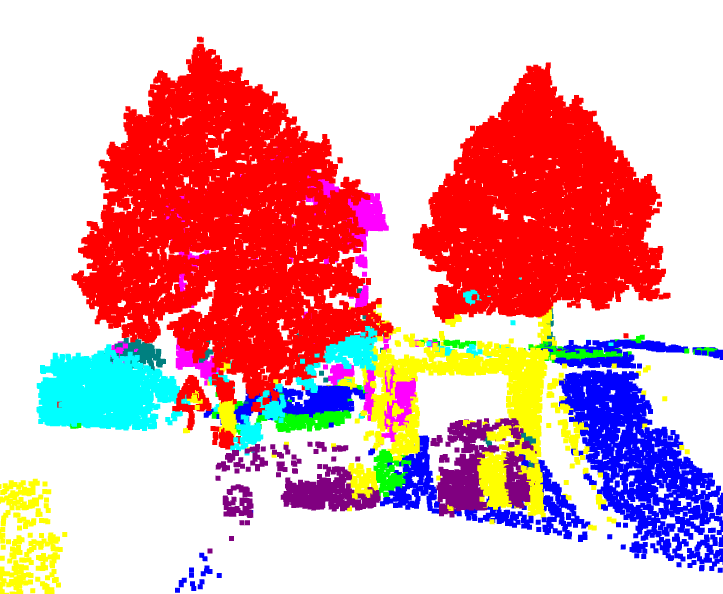
\includegraphics[width=0.30\textwidth, height=0.15\textheight]{images/seg_output/deep_ensembles/2_1.png} &
            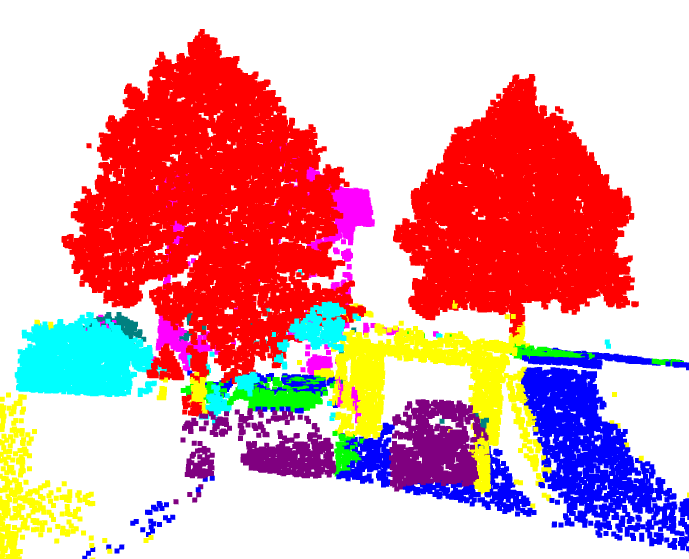
\includegraphics[width=0.30\textwidth, height=0.15\textheight]{images/seg_output/deep_ensembles/2_5.png}& 
            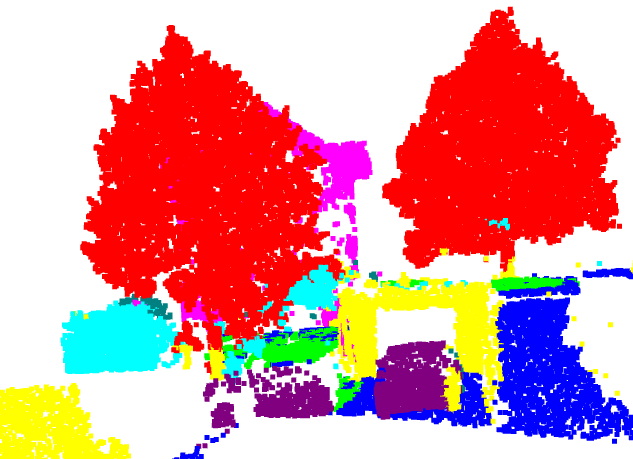
\includegraphics[width=0.30\textwidth, height=0.15\textheight]{images/seg_output/deep_ensembles/2_10.png}\\
        \end{tabular}
        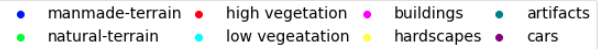
\includegraphics[scale=0.65]{images/legend.png}
        \caption{Deep ensembles performance on RandLA-Net over the Semantic3D dataset.}
        \label{fig:deepensemble_improv}
    \end{figure*}

    [Talk about lower class scores for some classes]
    From the Table~\ref{tab:ensemble_eval}, we infer that the Deep Ensembles improve the model's overall performance in terms of meanIoU and Accuracy.
    With an ensemble size of 10, we observe a 2\% increment in meanIoU.
    An increase in ensemble size also results in an improvement in per-class IoU performance.
    Figure~\ref{fig:deepensemble_improv} depicts the improvement in model classifications visually with the increase in ensemble size.
    From Figure~\ref{fig:deepensemble_vis_sem3d}, we also observe the misclassifications along the edges of the church, trees and ground.
    The possible explanation for these misclassifications is ambiguity in the feature vector of RandLA-Net. For example, a feature vector for the point along the lower edge of the church contains the part of ground points as the feature vector.
%%%%%%%%%%%%%%%%%%%%%%%%%%%%%%%%%%%%%%%%%%%%%%%%%%%%%%%%%%%%%%%%%%%%%%%%%%%%%%%
    \section{Flipout-Semantic3D}
    In this experiment, we trained a Flipout version of RandLA-Net as described in Section~[\$] over the Semantic3D dataset.
    Like Deep Ensembles, we performed 20 forward passes over the Flipout versioned RandLA-Net and averaged the predictions to obtain final predictions.
    Table~\ref{tab:flipout_eval} describes the performance of Flipout versioned RandLA-Net using meanIoU, per-class IoU and Accuracy.
    Figure~\ref{fig:flipout_vis_sem3d} depicts the predictions of the Flipout versioned RandLA-Net visually.
    \begin{table}[h!]
        \resizebox{\textwidth}{!}{%
        \begin{tabular}{c|c|cccccccc|c}
        %\textbf{\#Ensembles} & \textbf{MeanIOU} & \textbf{Accuracy} & \textbf{Manmadeterrain} & \textbf{Naturalterrain} & \textbf{Highvegetation} & \textbf{Lowvegetation} & \textbf{Buildings} & \textbf{Hardscapes} & \textbf{Scanningartifacts} & \textbf{Cars} \\ \hline
        & & \multicolumn{7}{c}{\textbf{IoU per class}} & \\ \hline
        \textbf{\#Passes} & \textbf{MeanIoU} & \textbf{C1} & \textbf{C2} & \textbf{C3} & \textbf{C4} & \textbf{C5} & \textbf{C6} & \textbf{C7} & \textbf{C8} & \textbf{Accuracy} \\ \hline
        1& 69.95  & 94.24&80.09&86.16&22.48&88.70&39.41&57.42&91.12&90.71\\
        5& 69.83  & 94.38&80.21&84.10&23.32&87.80&39.68&57.75&91.43&90.43\\
        10& 69.84 & 94.38&80.16&83.90&23.46&87.73&39.75&57.83&91.47&90.40\\
        15& 69.86 & 94.38&80.17&83.80&23.48&87.73&39.82&57.96&91.57&90.40\\
        20& 69.87 & 94.38&80.18&83.80&23.57&87.72&39.84&57.92&91.57&90.40\\
        \end{tabular}%
        }
        \caption{Illustration of performance of Flipout versioned RandLA-Net on Semantic3D. meanIOU and IOU per-class and overall accuracy are represented here.
        C1 to C8 are the classes of Semantic3D which are Manmadeterrain, Naturalterrain, Highvegetation, Lowvegetation, Buildings, Hardscapes, Scanningartifacts, and Cars.}
        \label{tab:flipout_eval}
    \end{table}
    \begin{figure*}[h!]
        \begin{tabular}{ccc}
            RGB & Ground Truth & Prediction-Flipout \\
            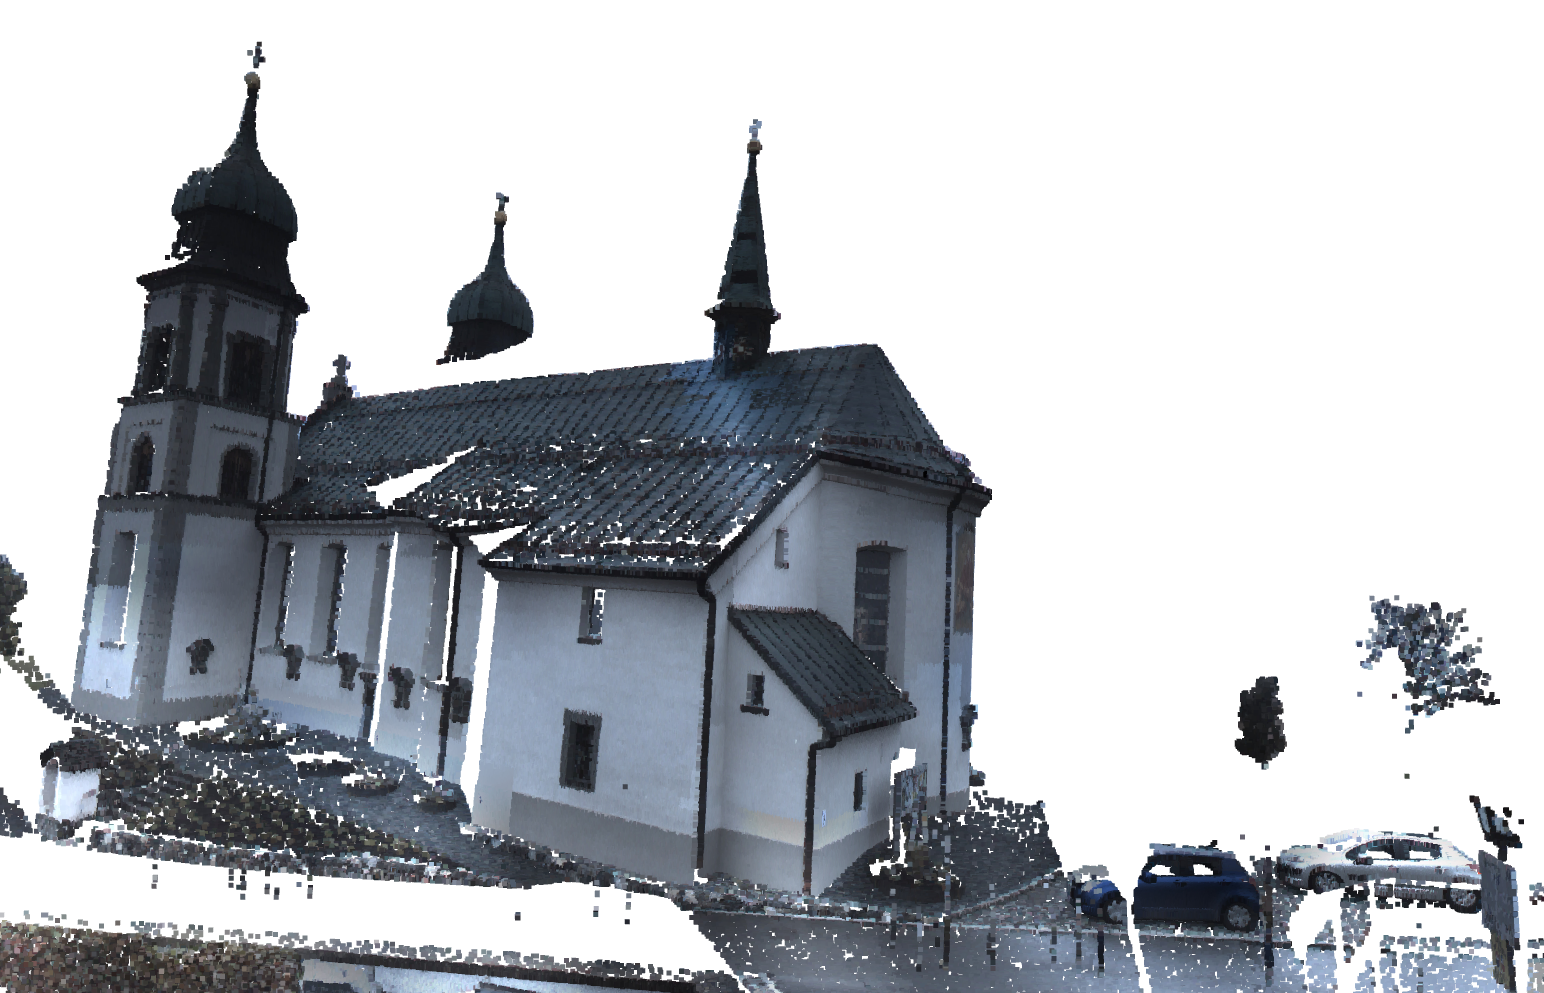
\includegraphics[width=0.33\textwidth, height=0.18\textheight]{images/seg_output/sem3d_seg_output/1_RGB.png} &
            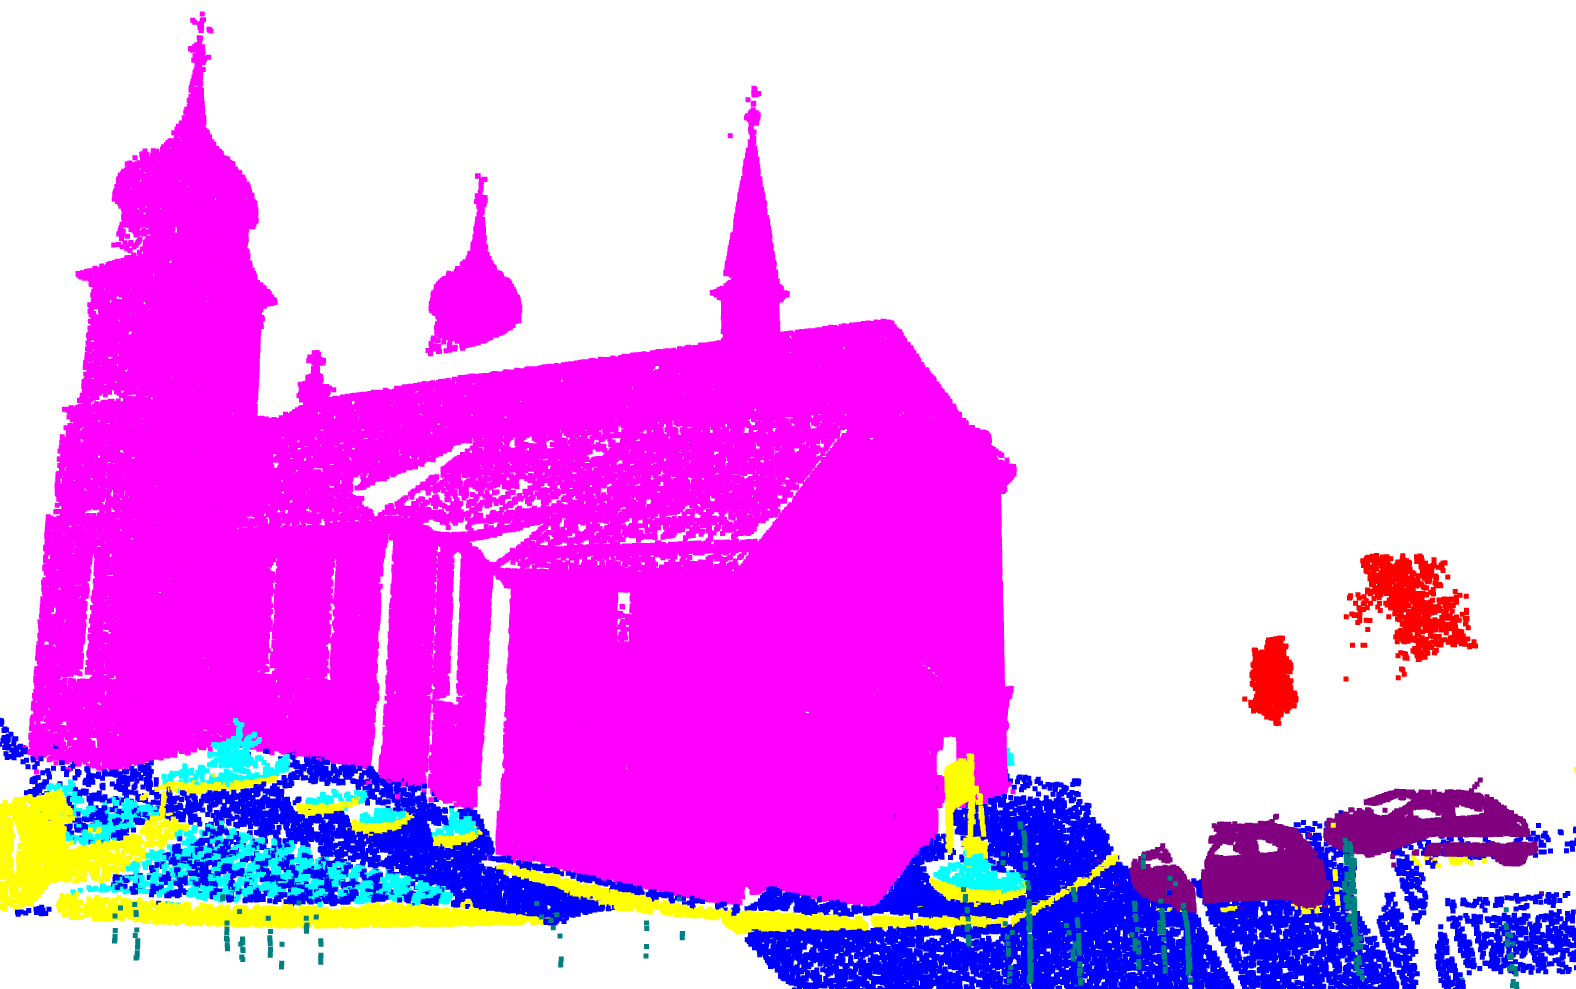
\includegraphics[width=0.33\textwidth, height=0.18\textheight]{images/seg_output/sem3d_seg_output/1_GT.png}& 
            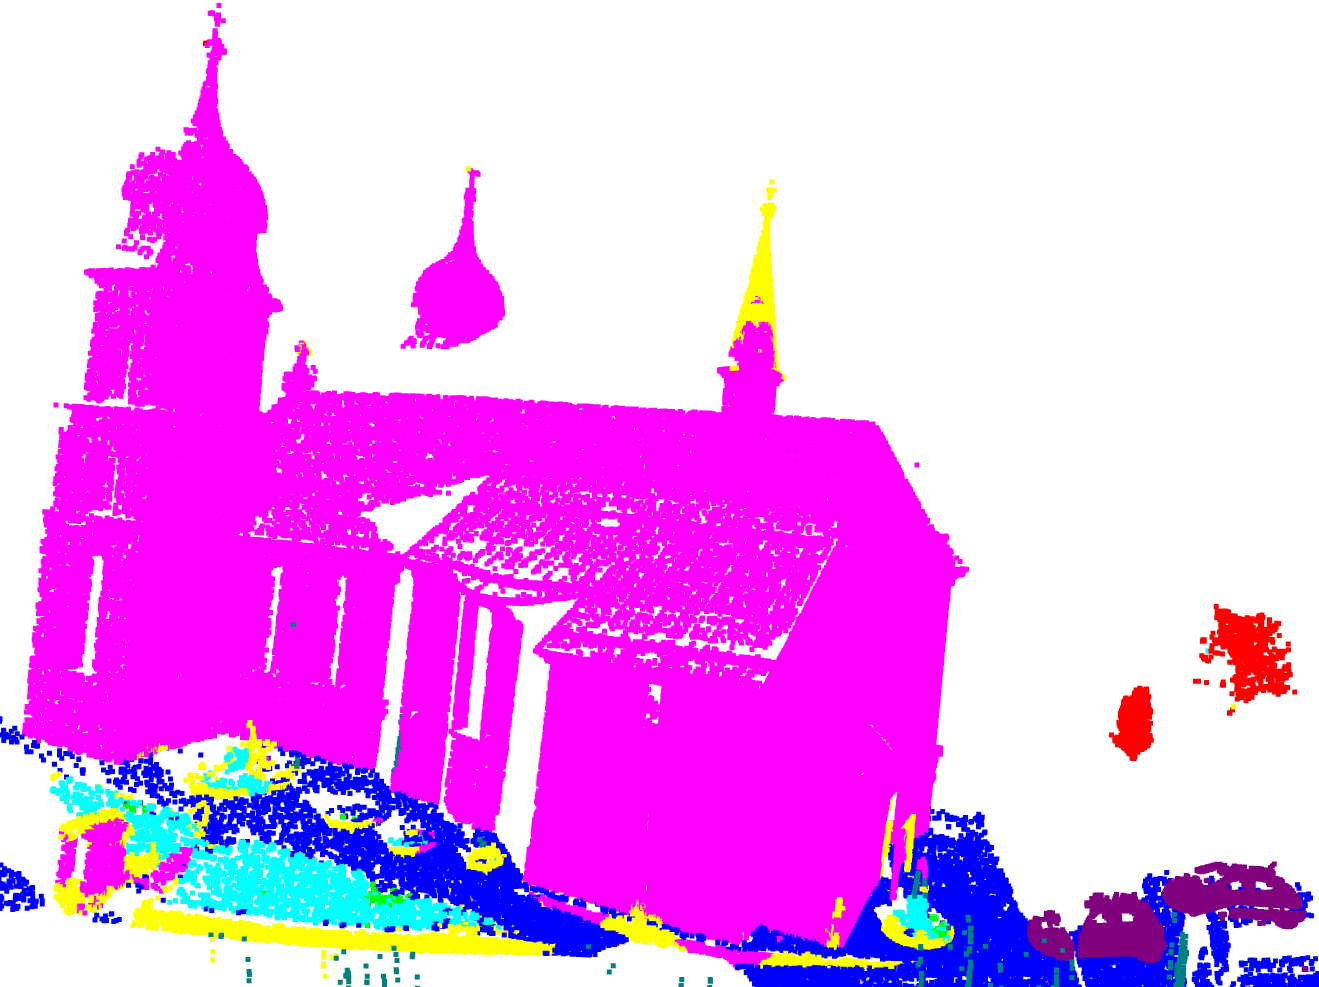
\includegraphics[width=0.33\textwidth, height=0.18\textheight]{images/seg_output/flipout/sem3d_1.png}\\

            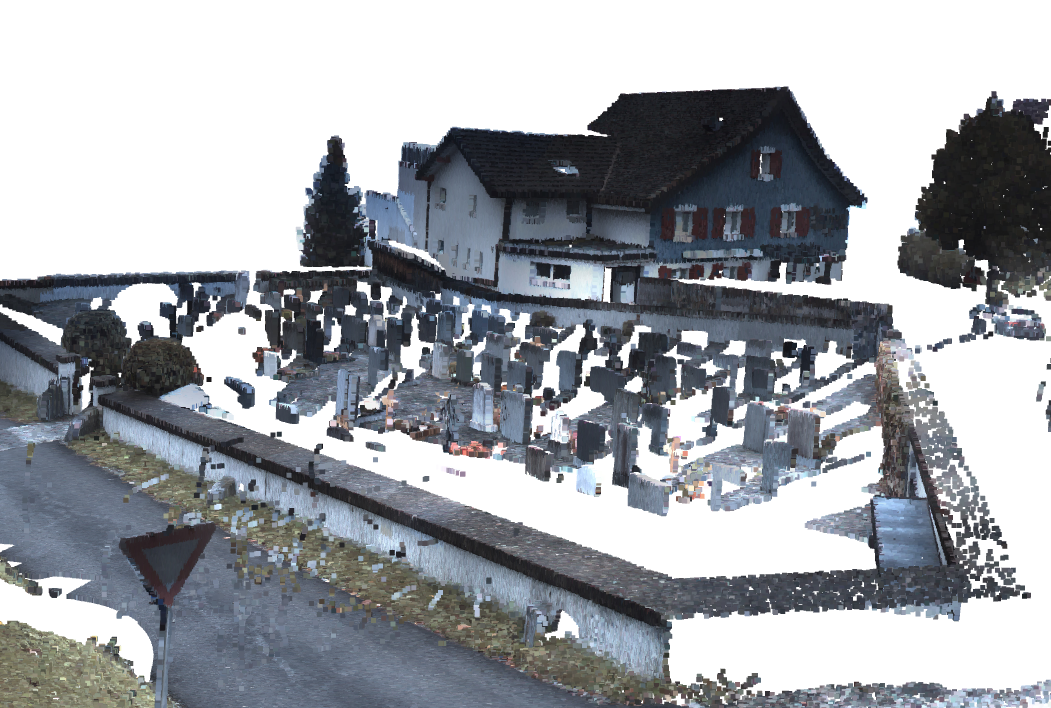
\includegraphics[width=0.33\textwidth, height=0.18\textheight]{images/seg_output/sem3d_seg_output/2_RGB.png} &
            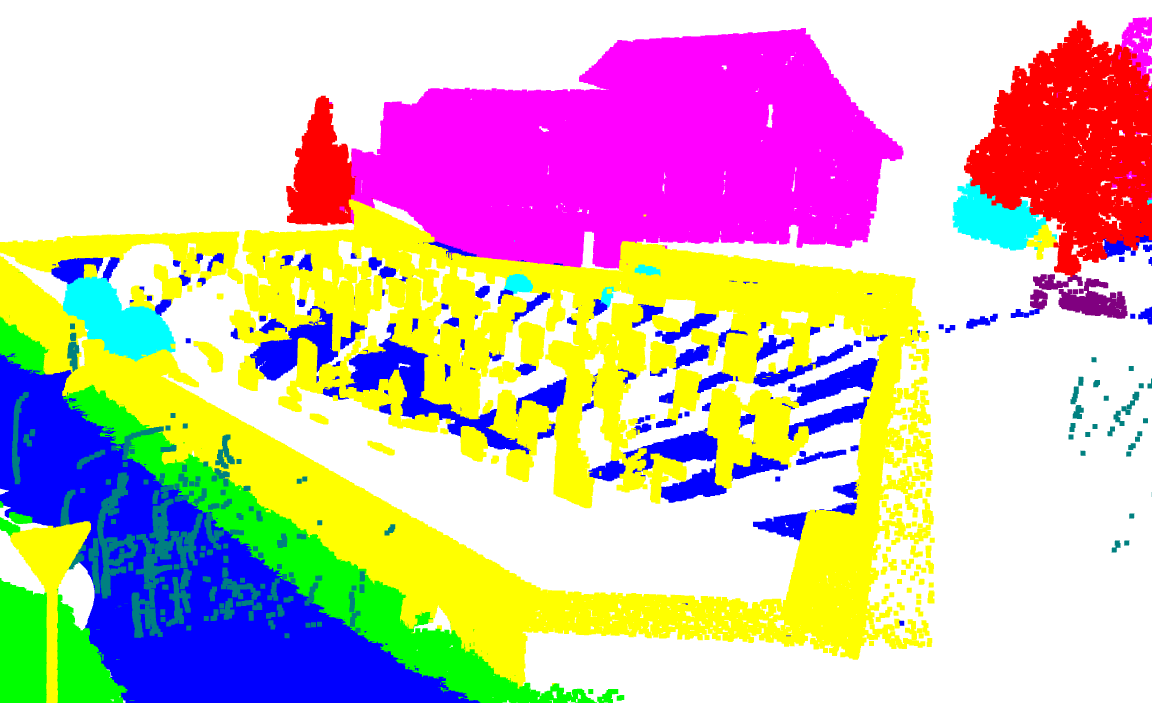
\includegraphics[width=0.33\textwidth, height=0.18\textheight]{images/seg_output/sem3d_seg_output/2_GT.png}& 
            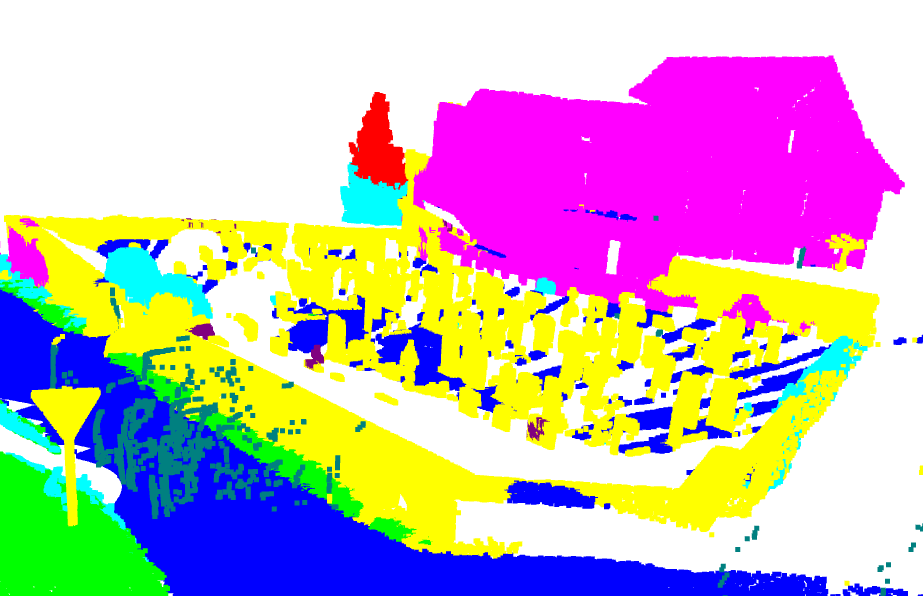
\includegraphics[width=0.33\textwidth, height=0.18\textheight]{images/seg_output/flipout/sem3d_2.png}\\

            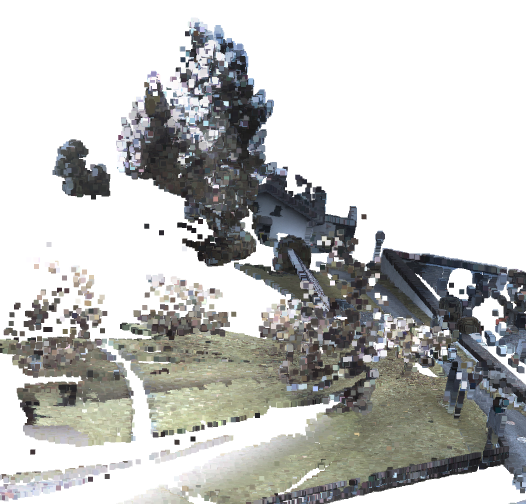
\includegraphics[width=0.33\textwidth, height=0.18\textheight]{images/seg_output/sem3d_seg_output/3_RGB.png} &
            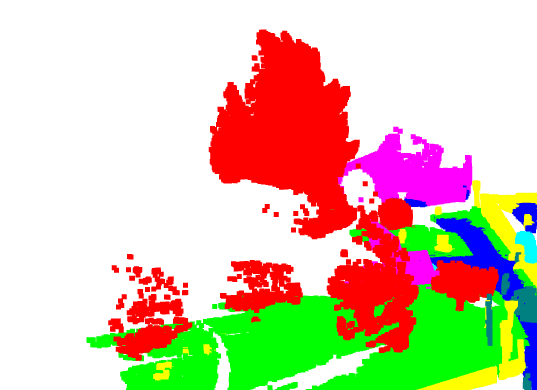
\includegraphics[width=0.33\textwidth, height=0.18\textheight]{images/seg_output/sem3d_seg_output/3_GT.png}& 
            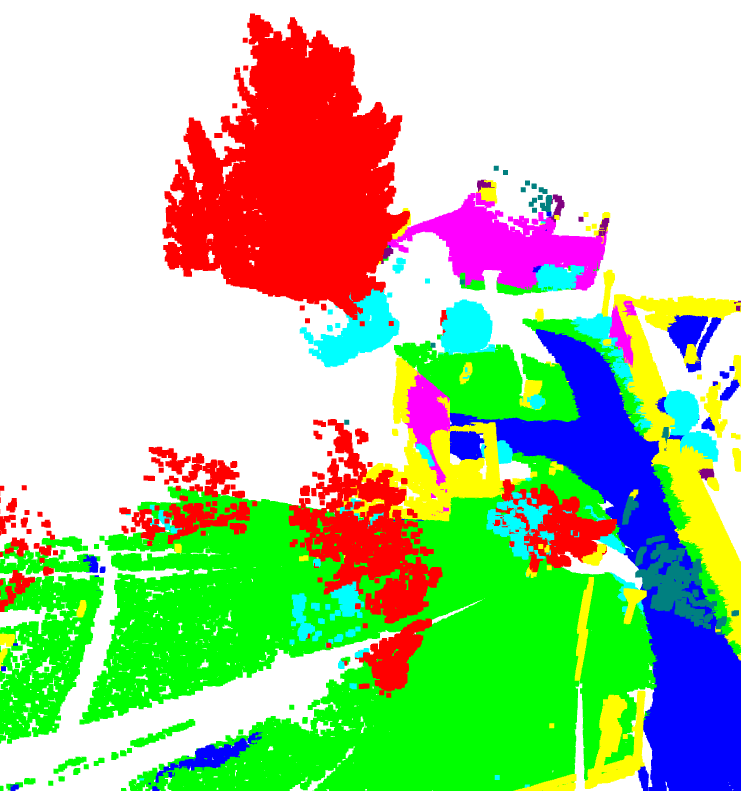
\includegraphics[width=0.33\textwidth, height=0.18\textheight]{images/seg_output/flipout/sem3d_3.png}\\
        \end{tabular}
        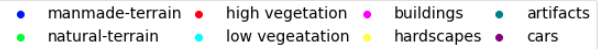
\includegraphics[scale=0.65]{images/legend.png}
        \caption{Output predictions of the RandLA-Net over the Semantic3D dataset (10 forward passes) \textcolor{red}{Legend spelling mistake}.}
        \label{fig:flipout_vis_sem3d}
    \end{figure*}   

    From Table~\ref{tab:flipout_eval}, we infer that the Flipout versioned RandLA-Net has a similar performance to the original RandLA-Net model proposed in \cite{Hu_2020_CVPR_Randla} and also Deep Ensembles with ensemble size one .
    We also observe a significant improvement in the Hardscapes class represented as C6 in Table~\ref{tab:flipout_eval}.
    There is a decrement in performance of classes Lowvegetation represented as C4 and Scanningartifacts represented as C7 in Table~\ref{tab:flipout_eval}, keeping the overall meanIoU same.
    % \textcolor{red}{Add the images of flipout performance here same as figures in deep ensembles}
    
%%%%%%%%%%%%%%%%%%%%%%%%%%%%%%%%%%%%%%%%%%%%%%%%%%%%%%%%%%%%%%%%%%%%%%%%%%%%%%%
    \section{OOD benchmark - Semantic3D vs S3DIS}
    In the previous section, we studied the performance of the Deep Ensembles and Flipout over the Semantic3D (In-Distribution) dataset.
    In this section, we study the predictions of the RandLA-Net model on the S3DIS (Out-Of-Distribution) dataset using Deep Ensembles and Flipout.
    We also compare the distribution of Maximum Softmax Probability (MSP) and entropy scores for Semantic3D and S3DIS datasets.

    Figure~\ref{fig:de_s3dis_vis} depicts the predictions of the RandLA-Net model and Flipout versioned RandLA-Net.
    We observe that most objects, such as ceilings and bookshelves, are labelled as buildings when using Deep Ensembles.
    We also observe that most point clouds are labelled as hardscapes class when using Flipout versioned RandLA-Net.
    The classifications on S3DIS datasets are in triangles because of the property of the scanner.
    As discussed in Section~[\$], data collected from the Matterport scanner is represented as triangular mesh, and then a point cloud is extracted from this mesh.

    \begin{figure*}[h!]
        \centering
        \begin{tabular}{ccc}
            RGB & Deep Ensembles & Flipout \\
            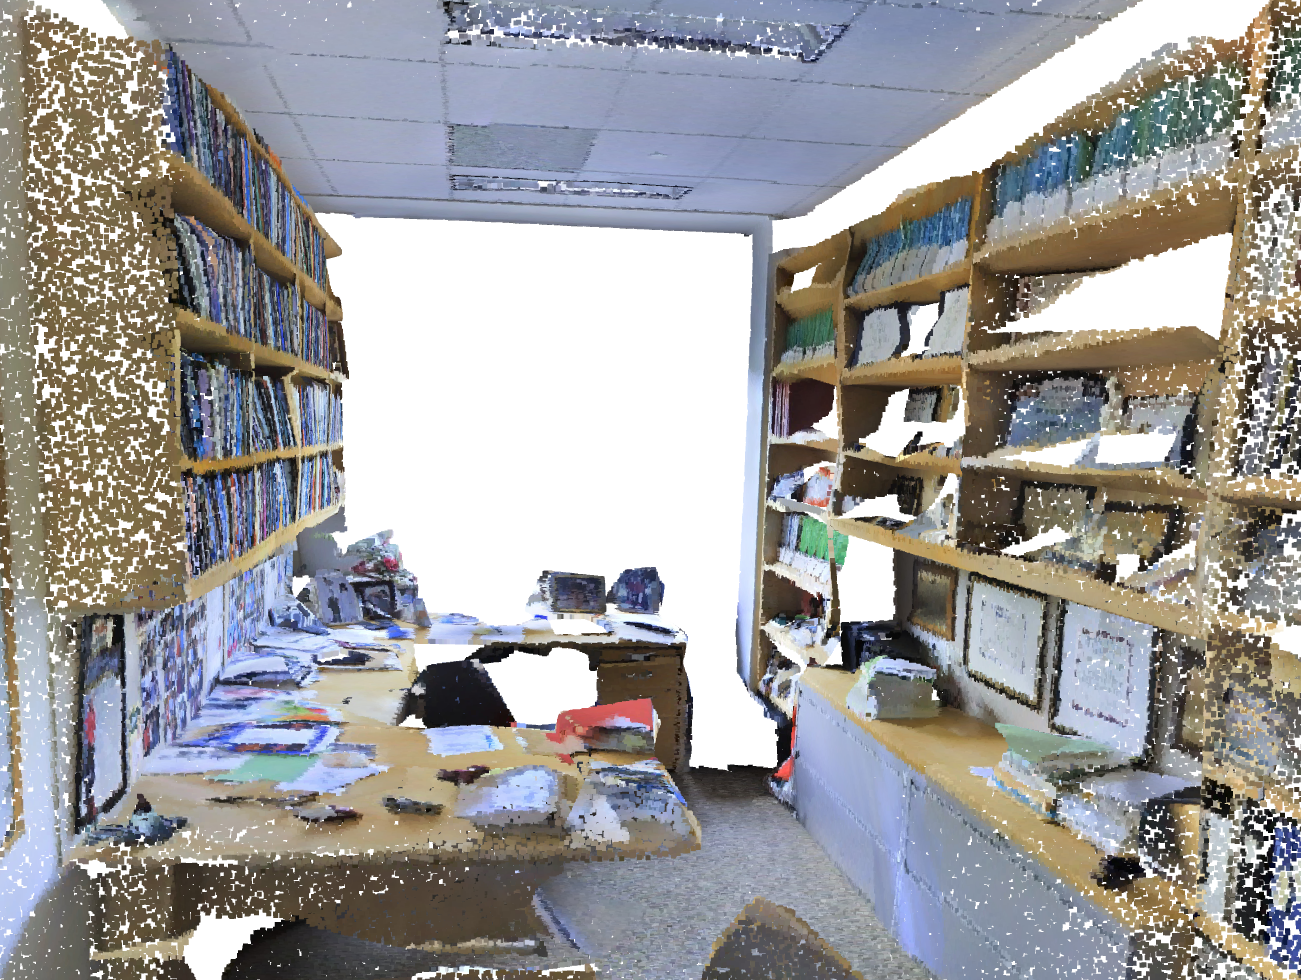
\includegraphics[width=0.33\textwidth, height=0.18\textheight]{images/seg_output/s3dis_DE/S3DIS_1_RGB.png} &
            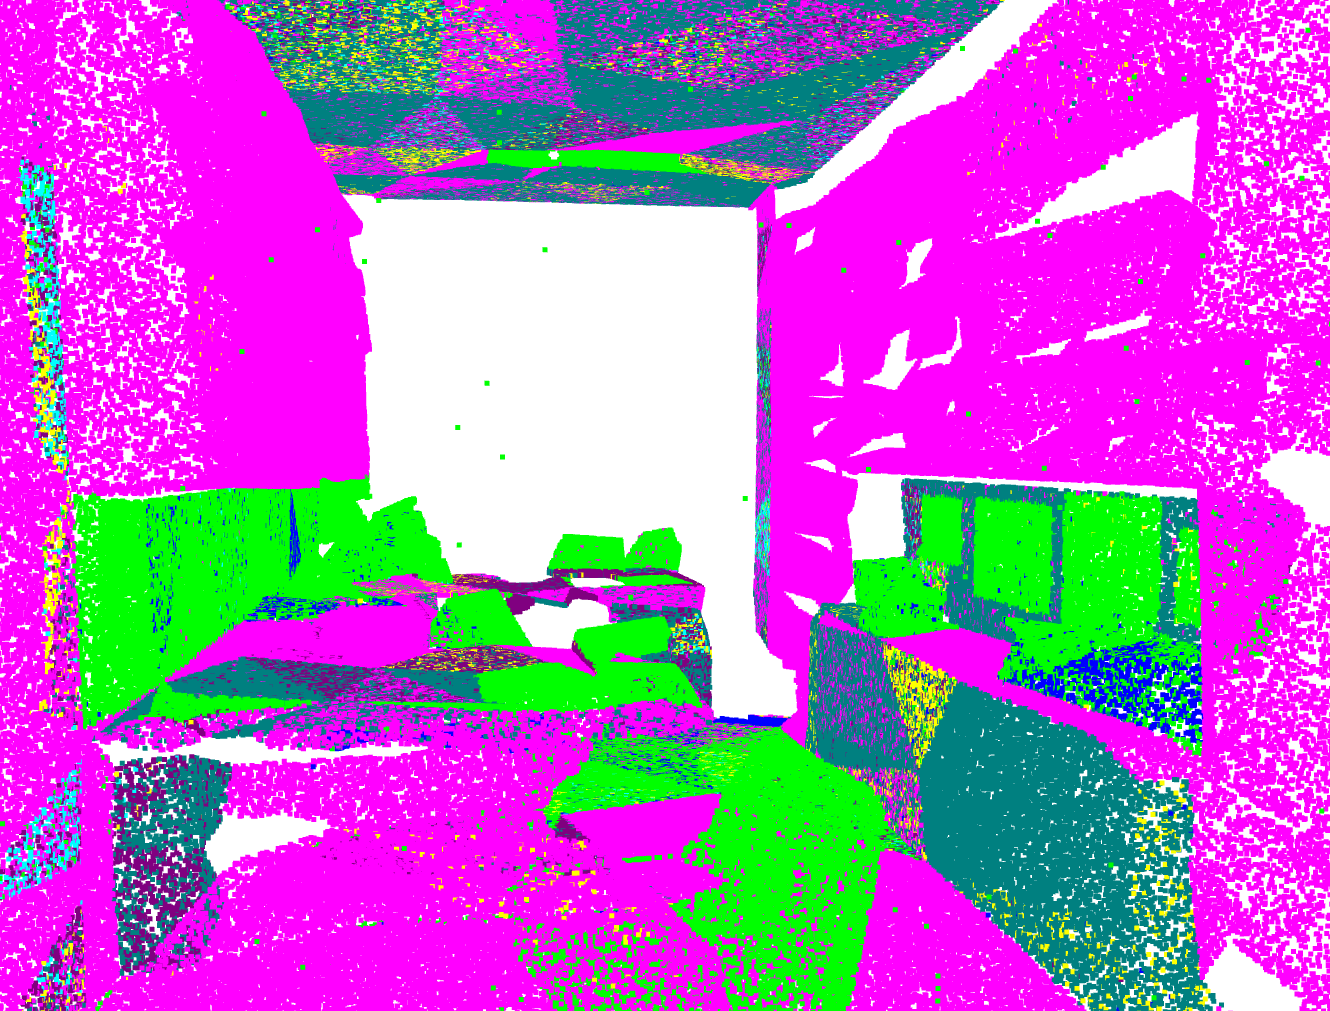
\includegraphics[width=0.33\textwidth, height=0.18\textheight]{images/seg_output/s3dis_DE/S3DIS_1_Pred.png} &
            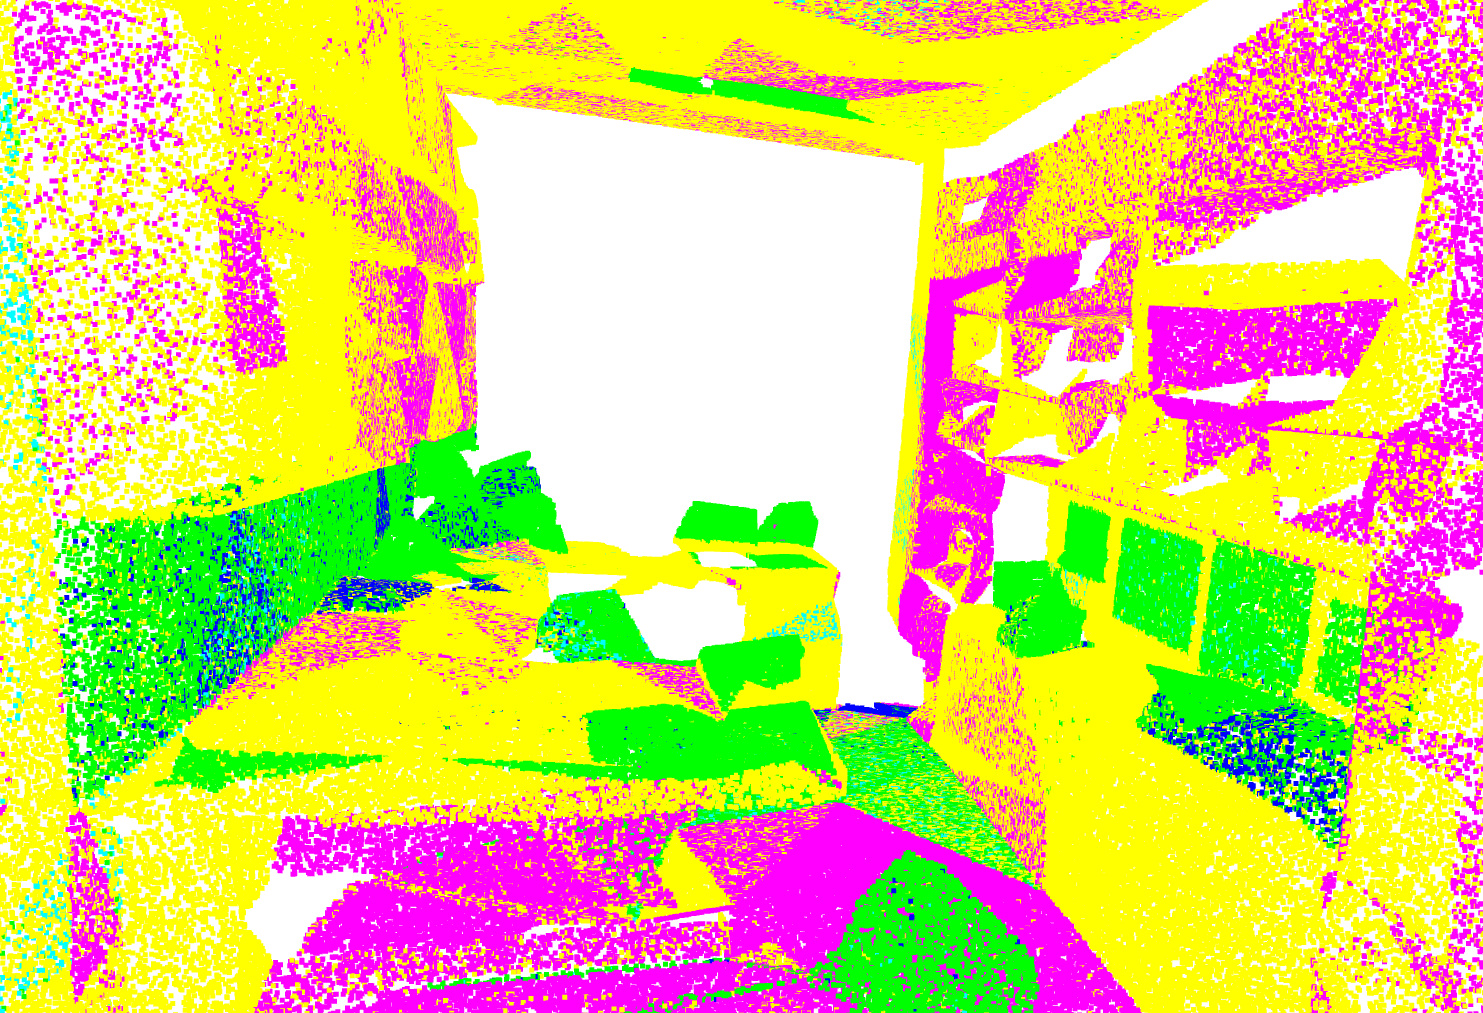
\includegraphics[width=0.33\textwidth, height=0.18\textheight]{images/seg_output/s3dis_DE/office_3.png} \\

            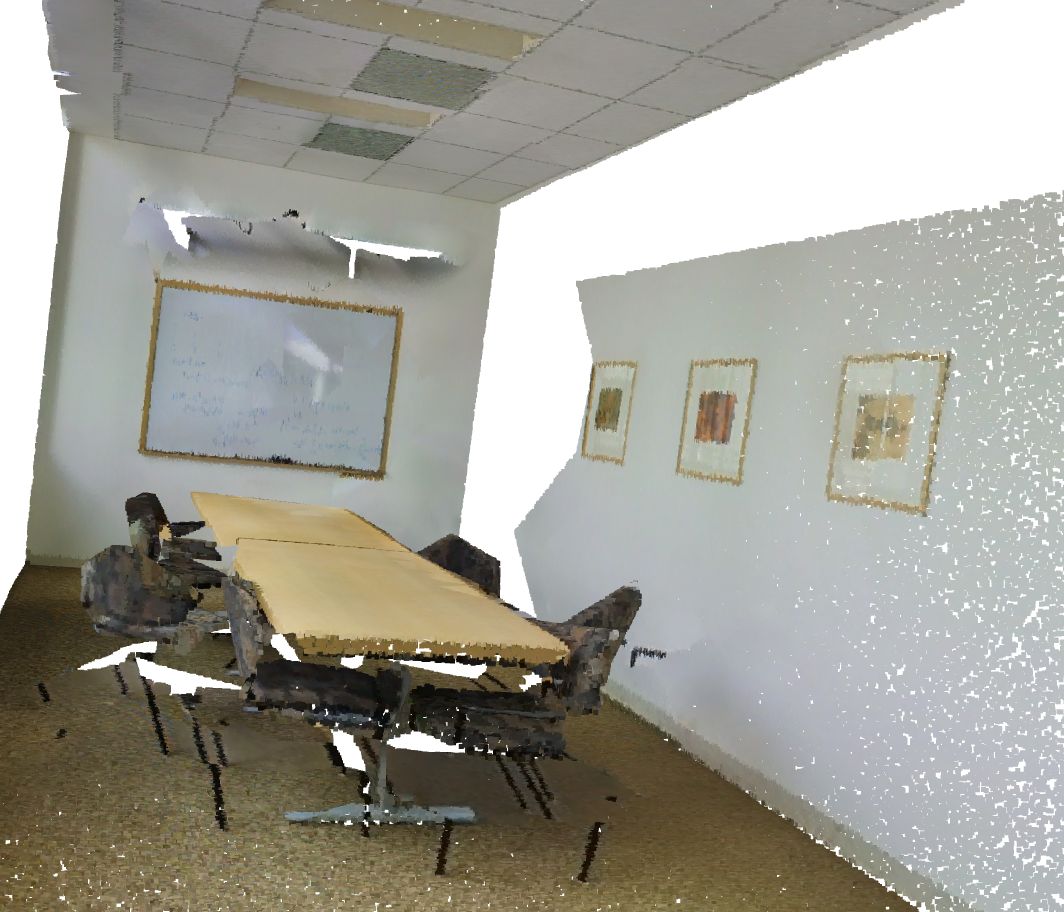
\includegraphics[width=0.33\textwidth, height=0.18\textheight]{images/seg_output/s3dis_DE/S3DIS_2_RGB.png} &
            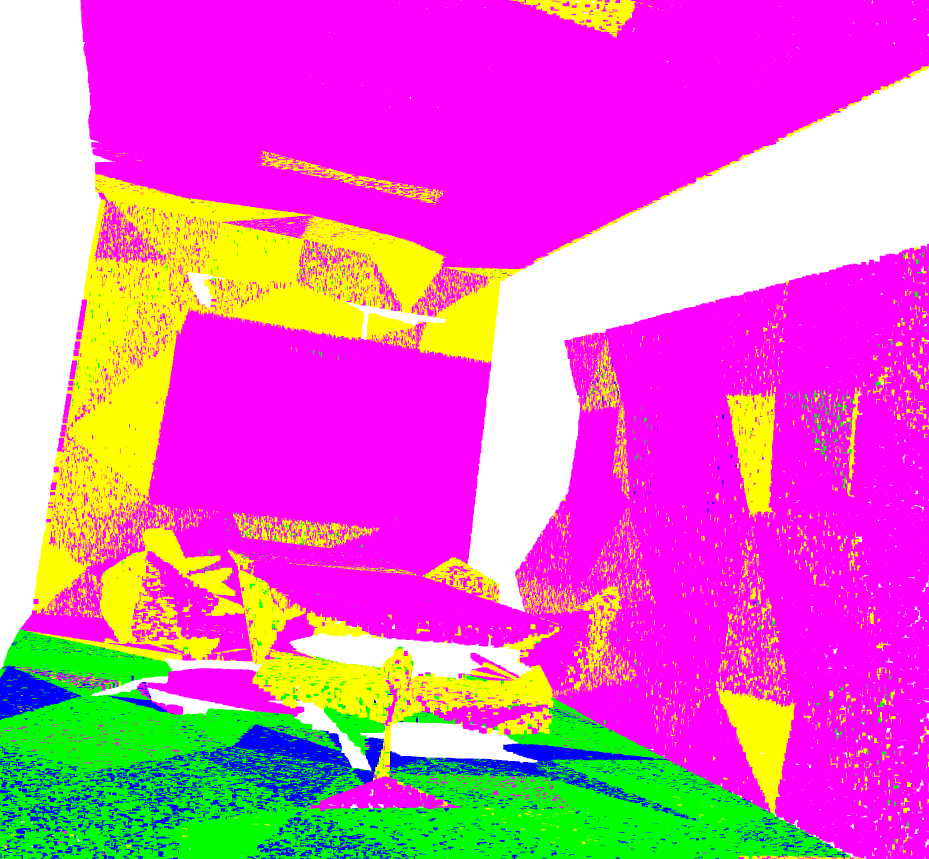
\includegraphics[width=0.33\textwidth, height=0.18\textheight]{images/seg_output/s3dis_DE/S3DIS_2_Pred.png}&
            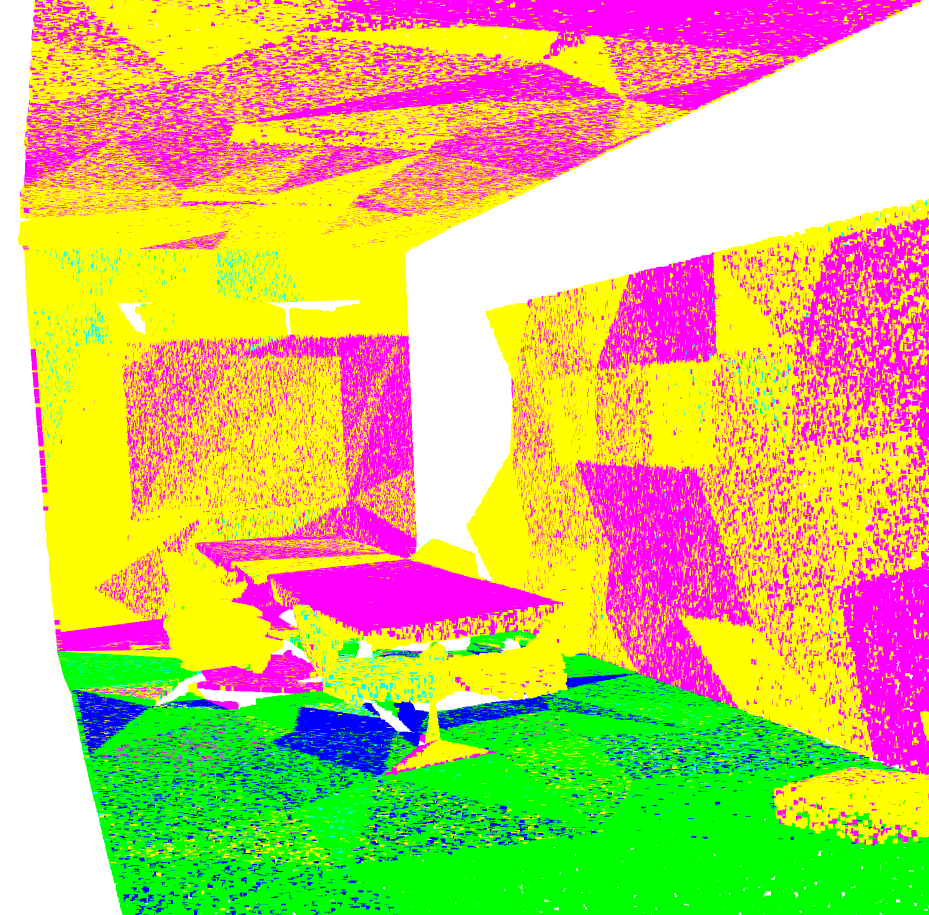
\includegraphics[width=0.33\textwidth, height=0.18\textheight]{images/seg_output/s3dis_DE/ocroom_1.png} \\
            
            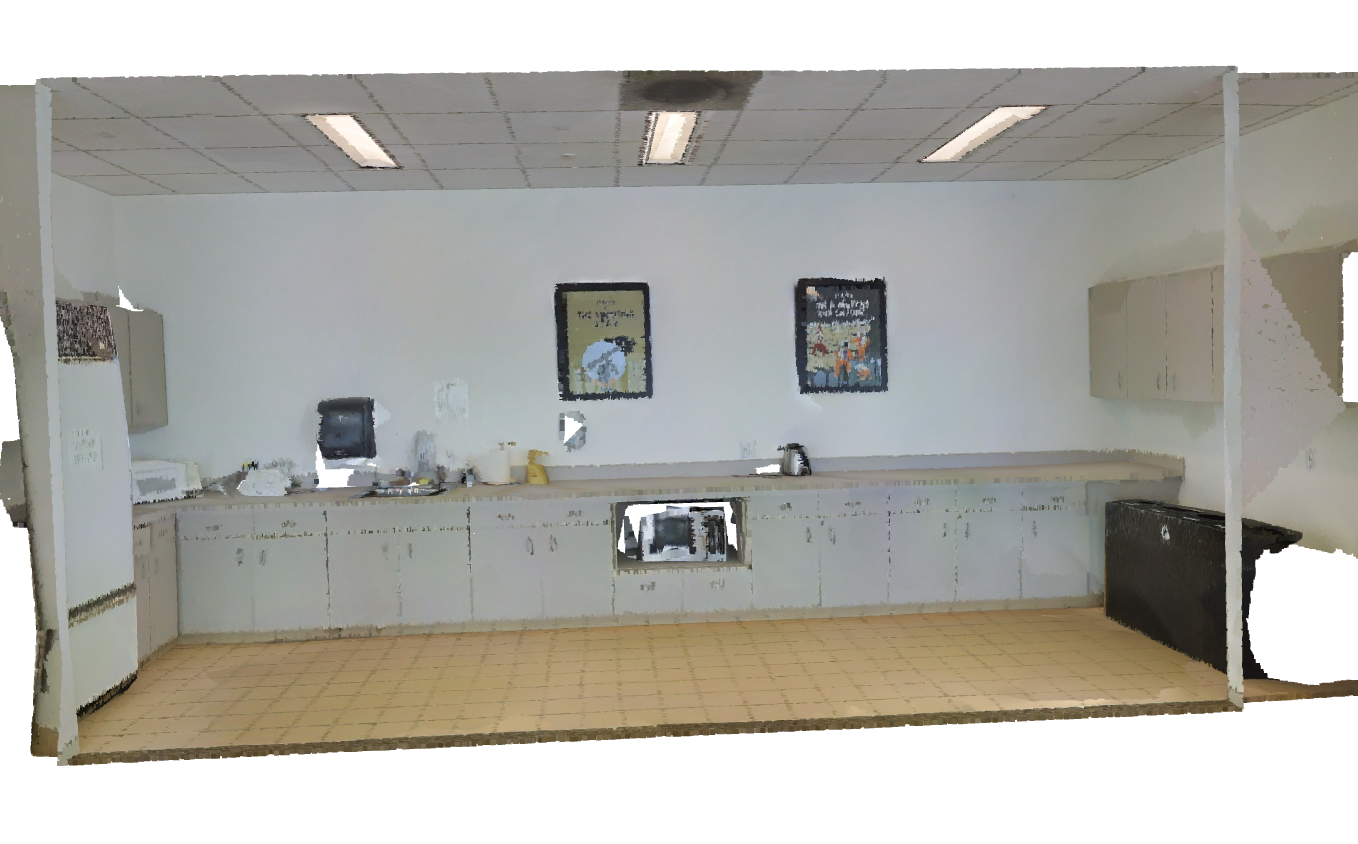
\includegraphics[width=0.33\textwidth, height=0.18\textheight]{images/seg_output/s3dis_DE/S3DIS_3_RGB.png} &
            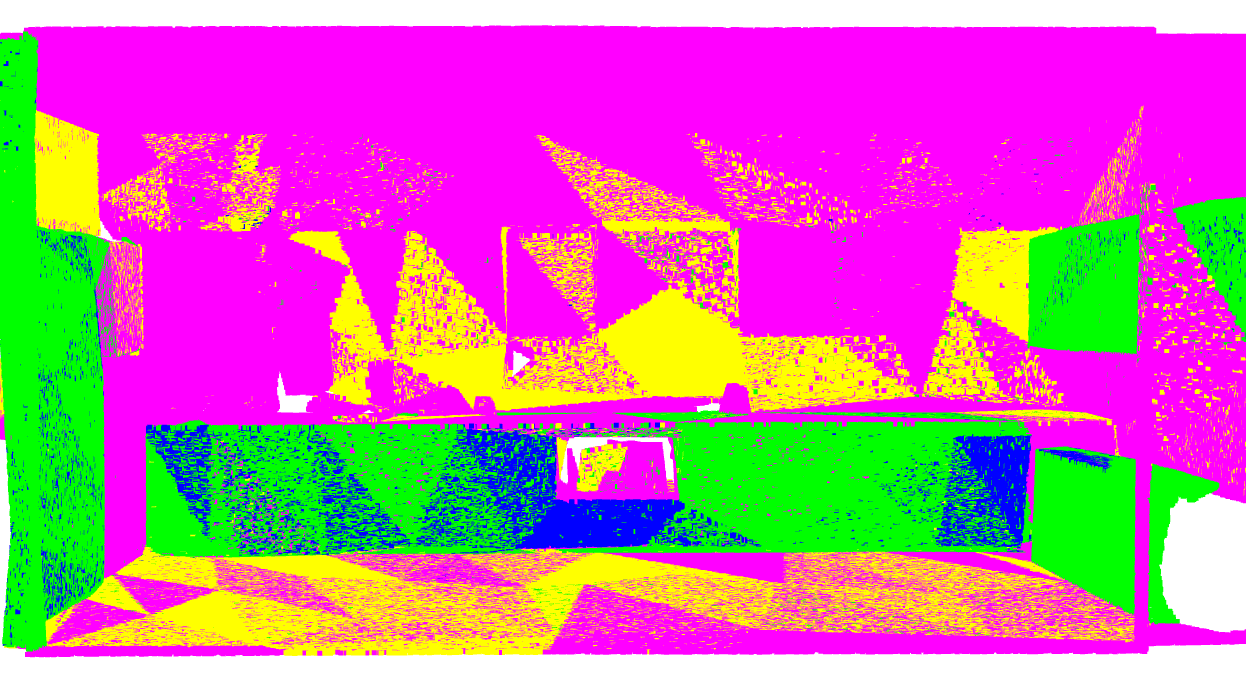
\includegraphics[width=0.33\textwidth, height=0.18\textheight]{images/seg_output/s3dis_DE/S3DIS_3_Pred.png}&
            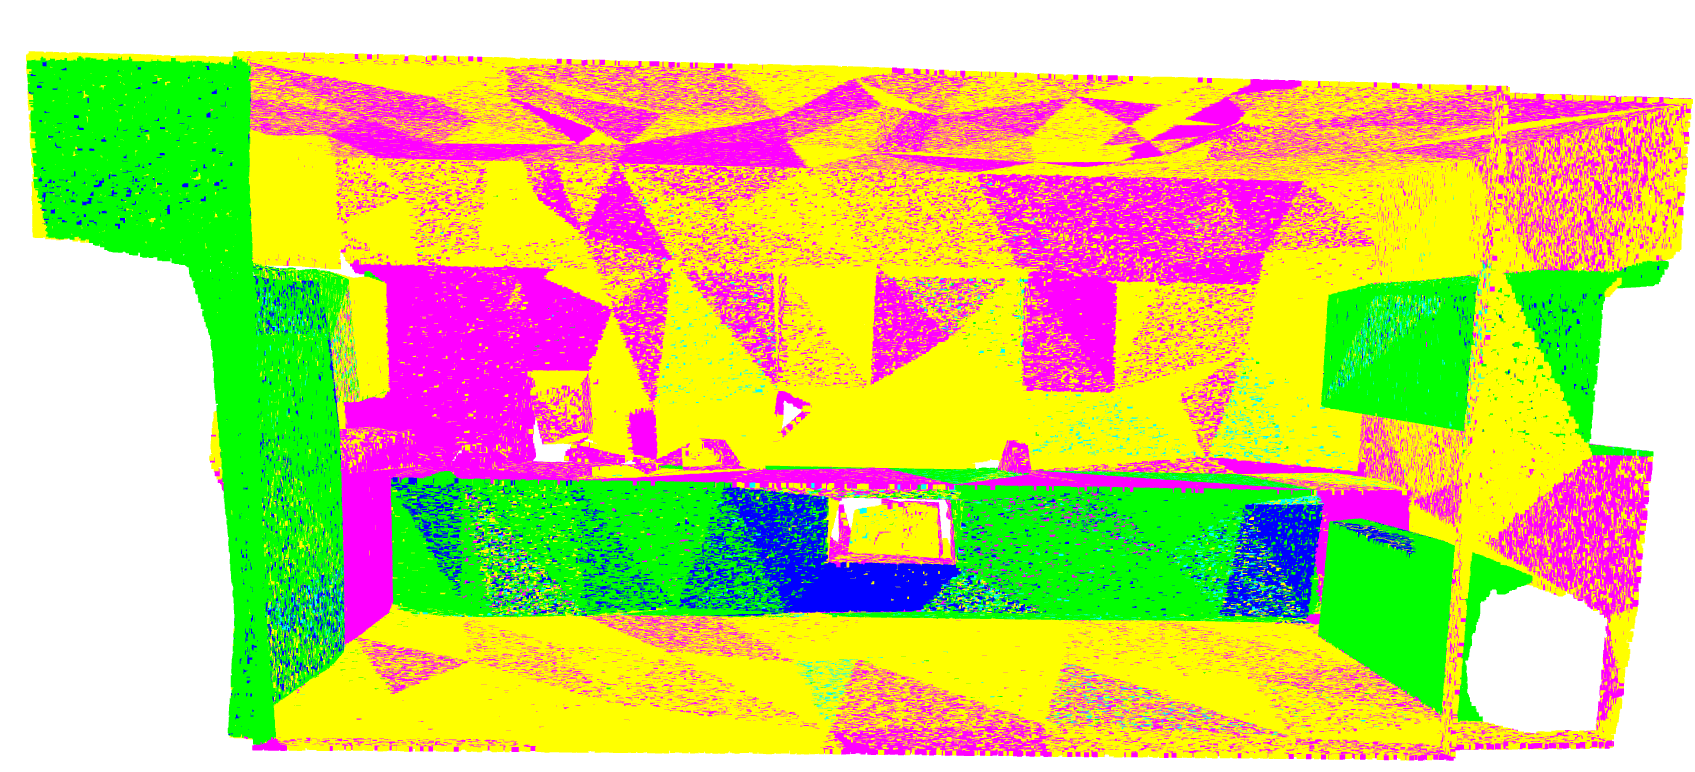
\includegraphics[width=0.33\textwidth, height=0.18\textheight]{images/seg_output/s3dis_DE/opantry_1.png} \\

            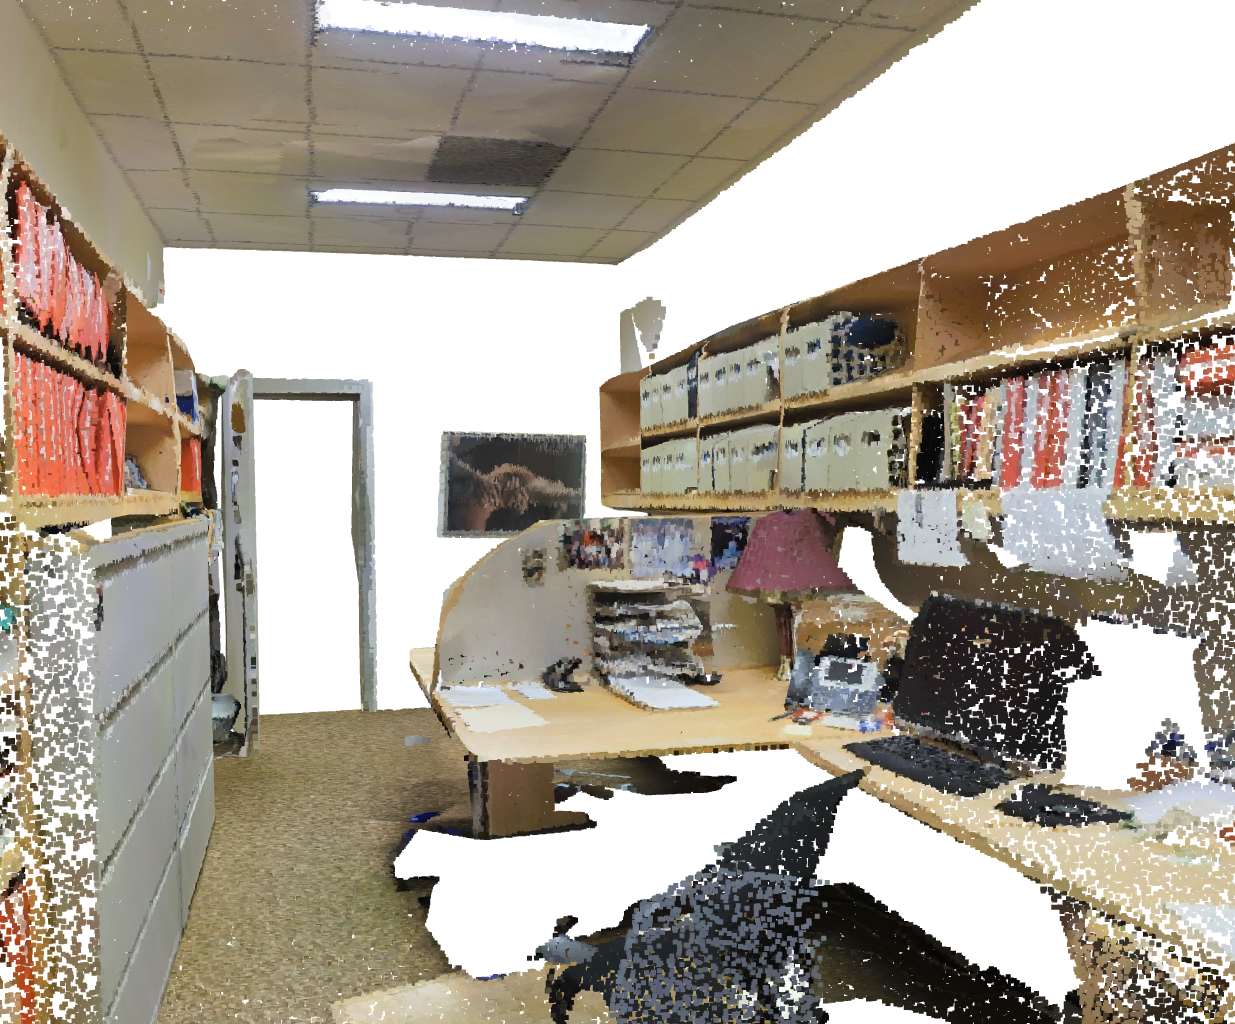
\includegraphics[width=0.33\textwidth, height=0.18\textheight]{images/seg_output/s3dis_DE/S3DIS_4_RGB.png} &
            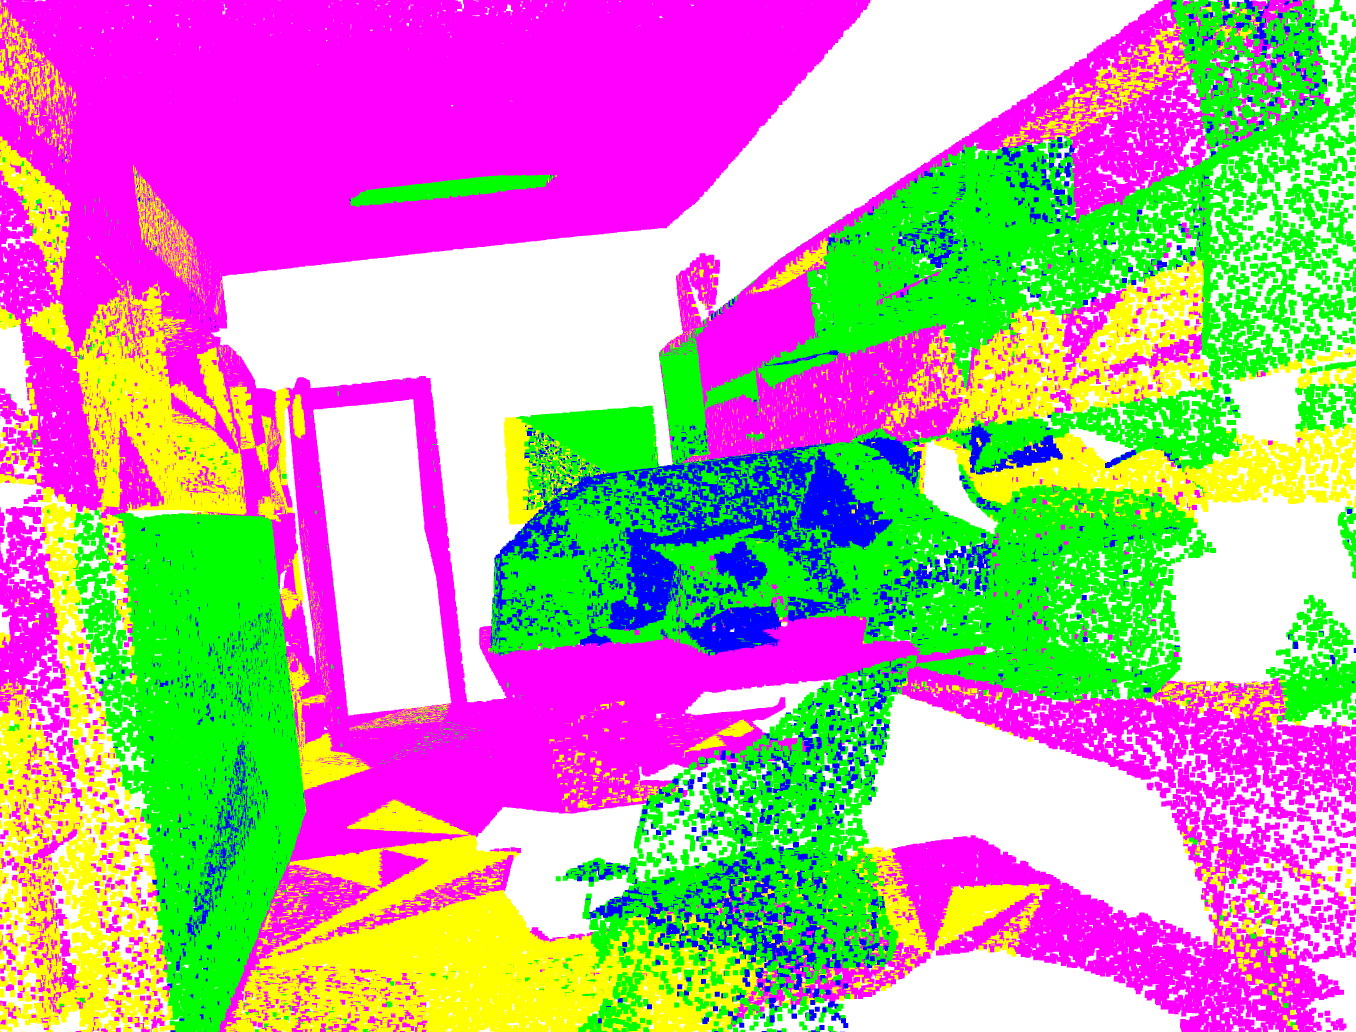
\includegraphics[width=0.33\textwidth, height=0.18\textheight]{images/seg_output/s3dis_DE/S3DIS_4_Pred.png}&
            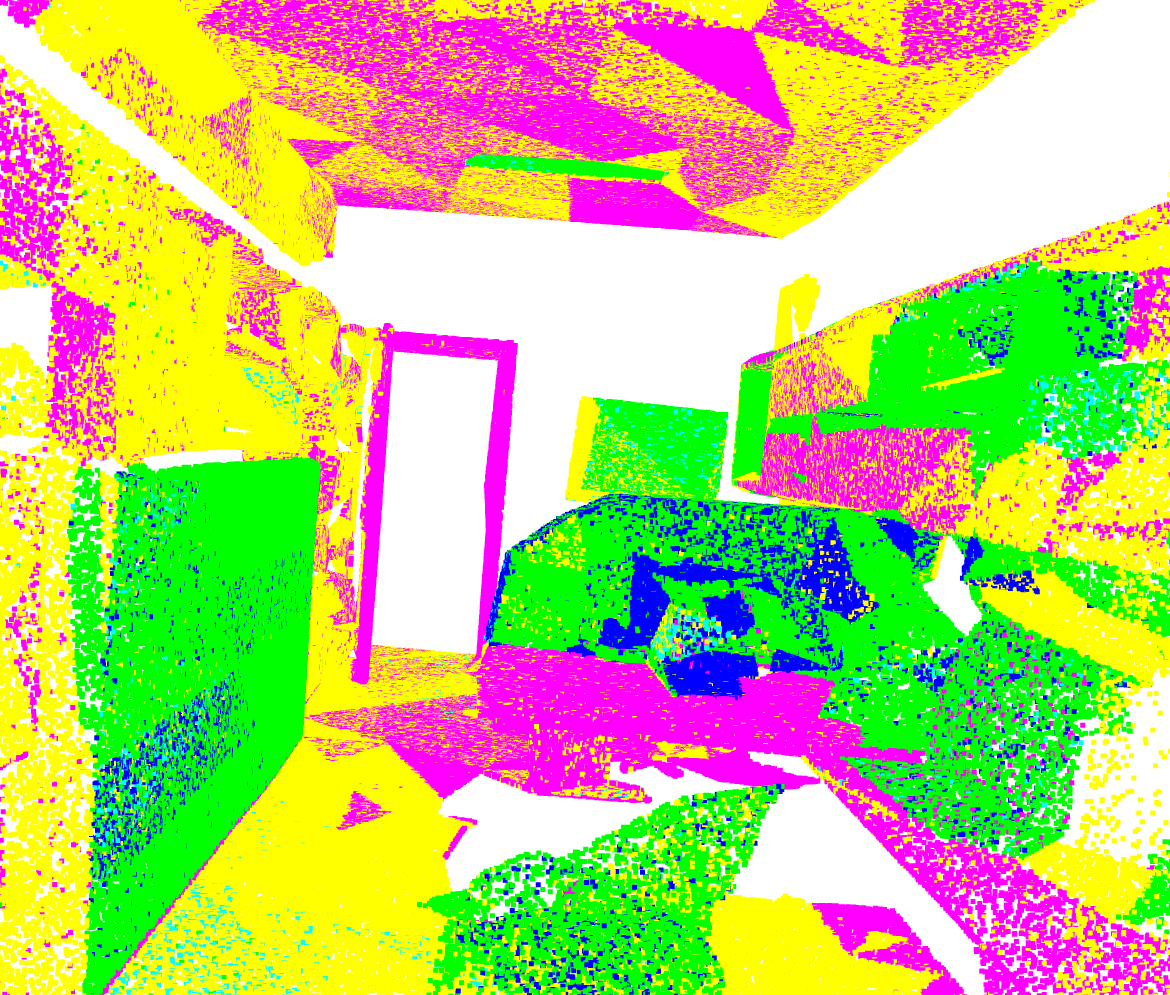
\includegraphics[width=0.33\textwidth, height=0.18\textheight]{images/seg_output/s3dis_DE/office_42.png} \\
        \end{tabular}
        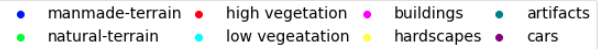
\includegraphics[scale=0.65]{images/legend.png}
        \caption{Output predictions of the RandLA-Net over the S3DIS dataset.}
        \label{fig:de_s3dis_vis}
    \end{figure*}
    %%%%%% Maximum probability (Semantic3D vs S3DIS) %%%%%%
    \subsection{Maximum Softmax Probability (MSP)}
    \label{sec:prob_sem3dvs3dis}
    In this experiment, we study the probability values of the ID dataset (Semantic3D), and OOD dataset (S3DIS) computed using Deep Ensembles and Flipout methods of RandLA-Net.
    We compute the average of the maximum softmax probability of all the points in the dataset, and this averaged value is called here the mean probability value.
    Figure~\ref{fig:msp_ensembles} and Figure~\ref{fig:msp_flipout} depicts the mean probability values across the ID (green) and OOD (red) datasets and their variance represented as error bars.
    Figure~\ref{fig:msp_ensembles} represents the change in mean probability value to ensemble size.
    Figure~\ref{fig:msp_flipout} represents the change in mean probability value to the number of passes in Flipout.
    Here, we represent the mean probability values across the odd number of ensembles size and the odd number of passes in case of flipout.
    \begin{figure}[!ht]
        \centering
        \begin{subfigure}{0.98\textwidth}
        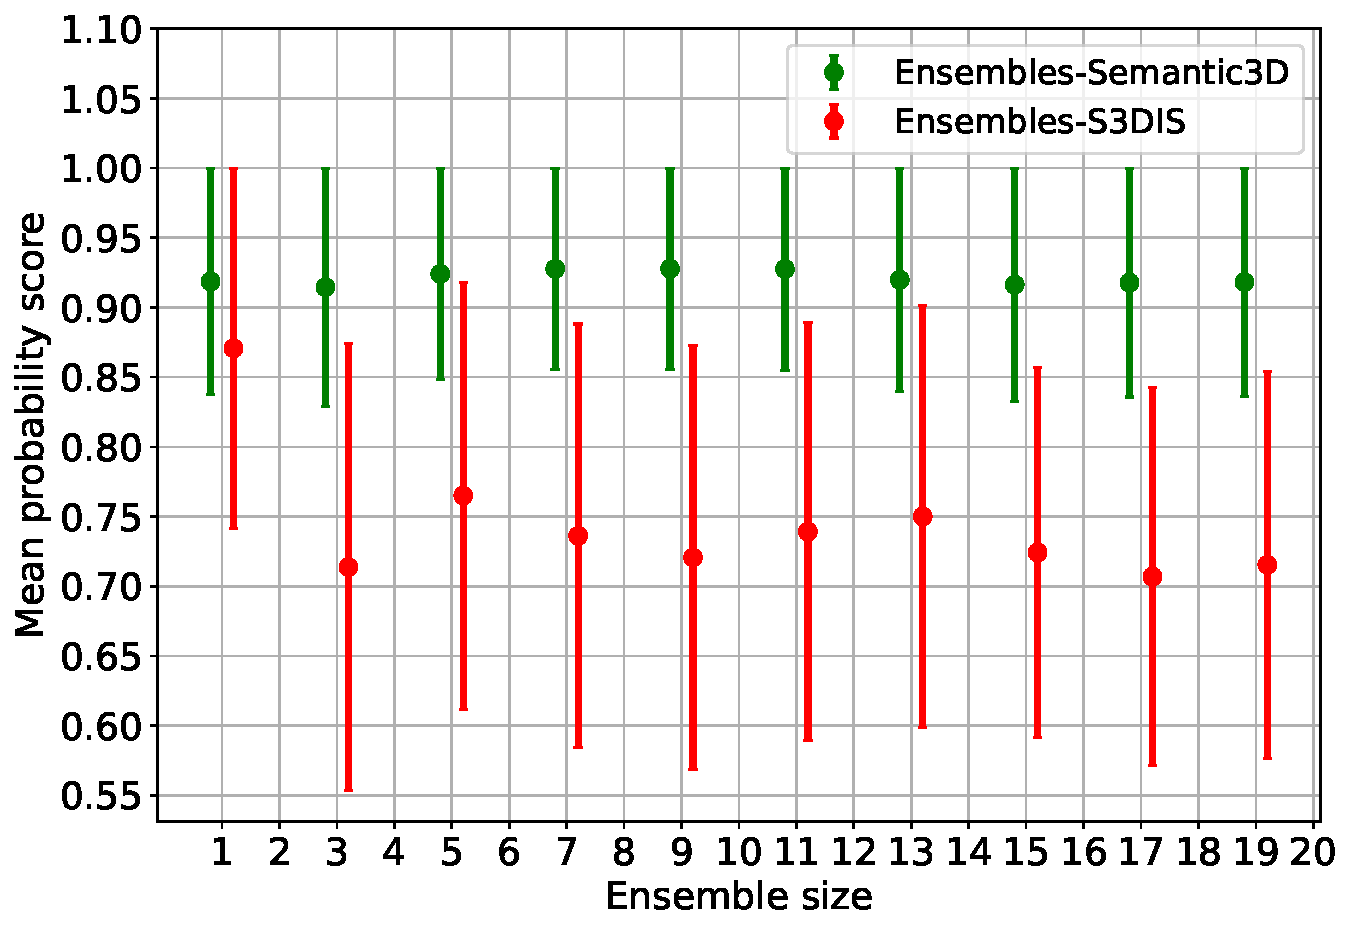
\includegraphics[scale=0.6]{images/MSP/Ensembles_MSP_cnc.pdf}
        \caption{MSP deep ensembles}
        \label{fig:msp_ensembles}
        \end{subfigure}
        \begin{subfigure}{0.98\textwidth}
        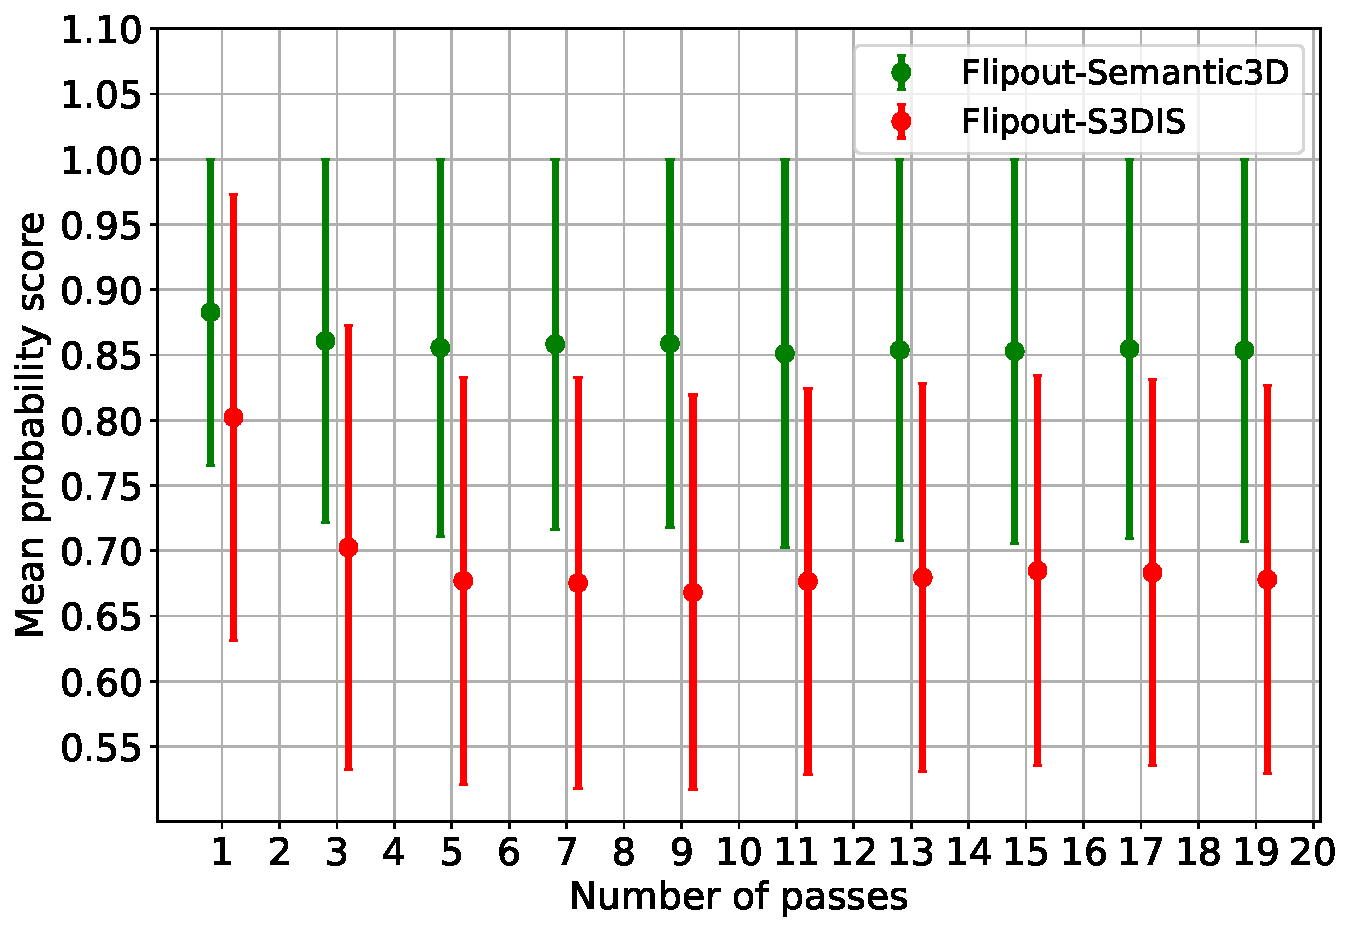
\includegraphics[scale=0.6]{images/MSP/Flipout_MSP_cnc.pdf}
        \caption{MSP flipout}
        \label{fig:msp_flipout}
        \end{subfigure}
    \end{figure}

    From Figure~\ref{fig:msp_ensembles}, we can infer that as the increase in ensemble size, the mean probability of the ID (Semantic3D) dataset remains stable.
    The variance is reduced until the ensemble size of 9 and then stabilizes.
    In the case of the OOD (S3DIS) dataset, we observe a decrement in mean probability value and then remain the same after an ensemble size of 3 with a larger variance.
    With the increase in ensemble size, we also observe that the overlap in the variance of ID and OOD is getting lower.
    This smaller overlap in higher ensemble size should result in higher OOD detection performance.
    In the case of Flipout, as in Figure~\ref{fig:msp_flipout} the mean probability and variance remain mostly the same for the ID dataset.
    With the OOD dataset, we observed a reduction in the mean probability value in the case of multiple passes.
    The variance from the Flipout is higher than the Deep Ensembles for the ID dataset.
    This phenomenon is to be expected because the Deep Ensembles combine predictions from various radomly initializated models and in the case of Flipout same model is used for multiple forward passes.

    Figure~\ref{fig:de_sem3d_probmap} and Figure~\ref{fig:fout_sem3d_probmap} represent the ground truth, prediction and probability map of the ID (Semantic3D) dataset using Deep Ensembles and Flipout respectively.
    Similarly Figure~\ref{fig:de_s3dis_probmap} and Figure~\ref{fig:fout_s3dis_probmap} depict the prediction and probability map for OOD (S3DIS) dataset using Deep Ensembles and Flipout respectively.
    On visual inspection of Figure~\ref{fig:de_sem3d_probmap} and Figure~\ref{fig:fout_sem3d_probmap}, we observed that the probability scores are low for points which are misclassified.
    The points which lie on the edge of the structures are low scored.
    This effect is profound near the edges of church, and also edges of walls.
    In case of OOD dataset presented in Figure~\ref{fig:de_s3dis_probmap} and Figure~\ref{fig:fout_s3dis_probmap}, the overall probability scores are low, as the whole point cloud has greener shade than the ID dataset probability map represented in yellow shade.
    % \textbf{Aim: } In this experiment, we study how the probability scores are distributed in Semantic3D and S3DIS datasets which are ID and OOD datasets respectively.
    % \begin{figure}[h!]
    %     \centering
    % %\begin{subfigure}{0.54\textwidth}
    % %        \includestandalone[scale=0.9]{images/mean_prob_sem3dvs3dis}
    %     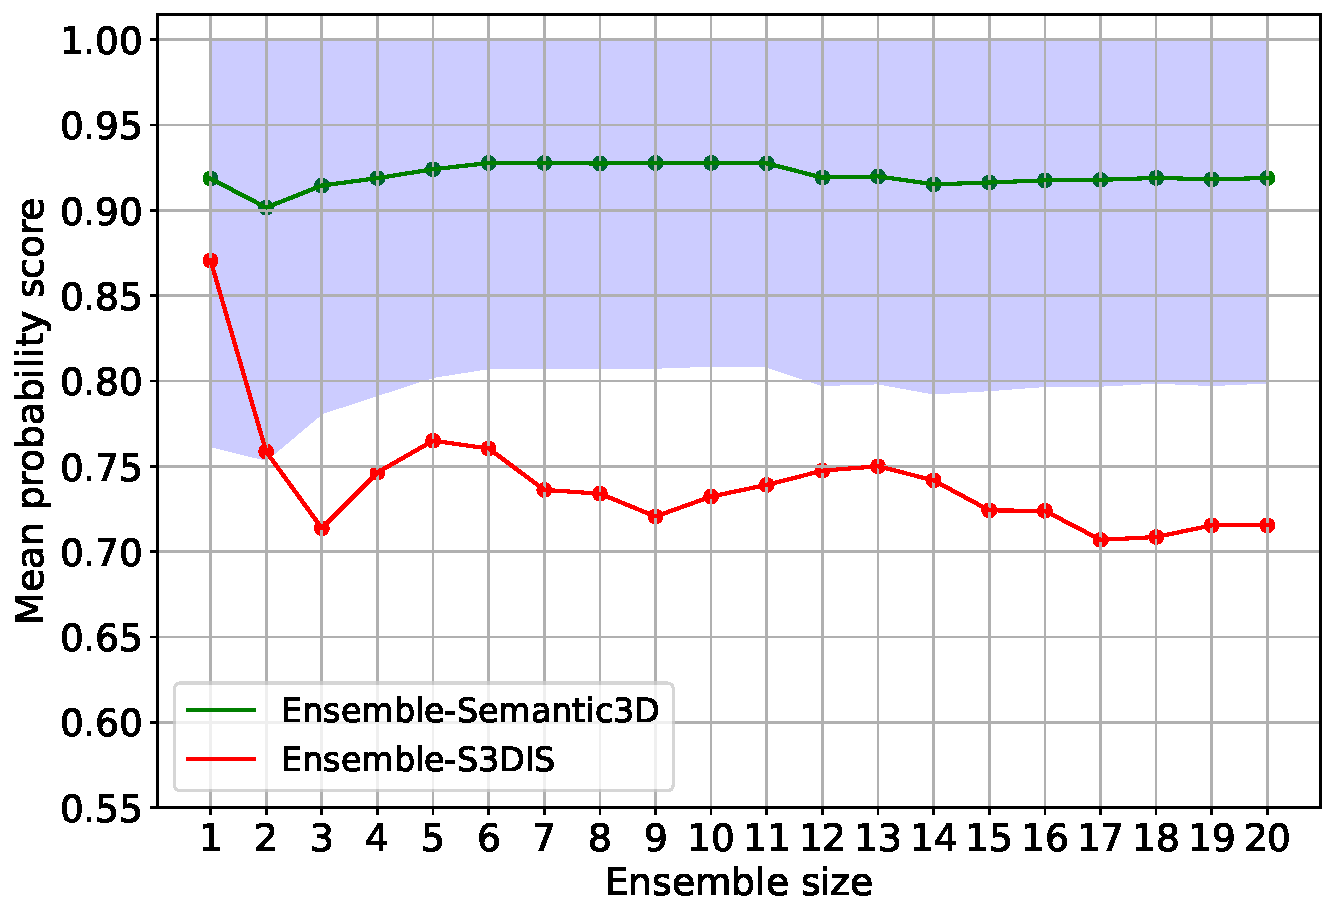
\includegraphics[scale=0.55]{images/Ensemble_MSP.pdf}
    %     \caption{}
    %     \label{fig:prob_sem3dvs3dis_de}    
    % %\end{subfigure}
    % \end{figure}
    % \begin{figure}[h!]
    %     \centering
    % %\begin{subfigure}{0.45\textwidth}
    % %       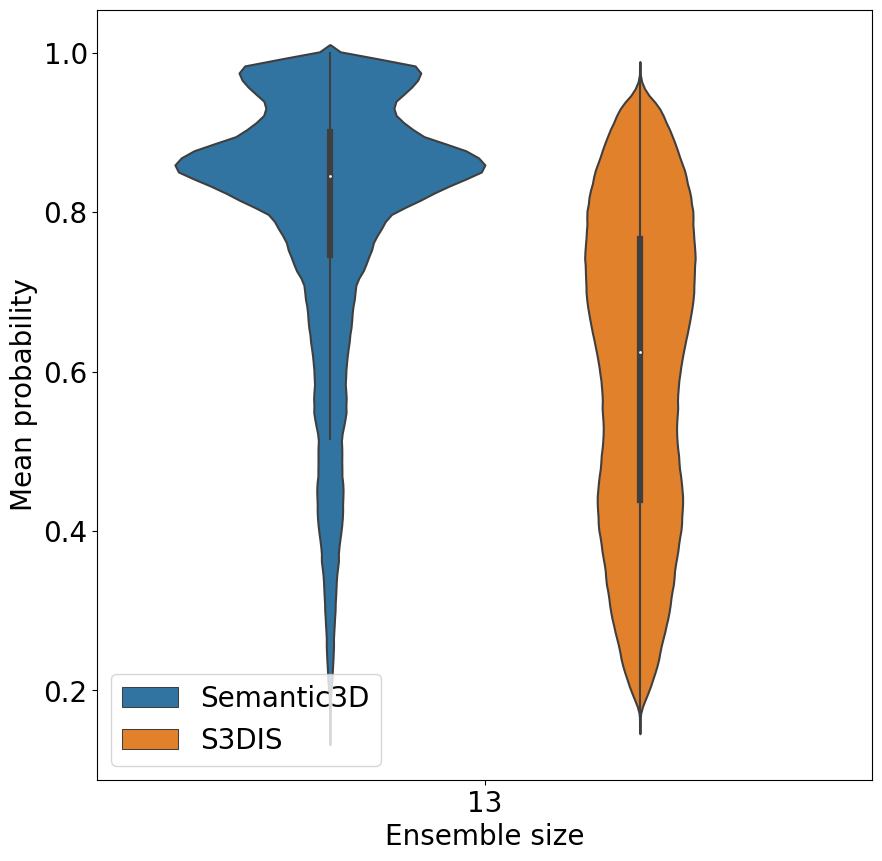
\includegraphics[scale=0.33]{images/violin_in_Max_predicted_probability.png}
    %     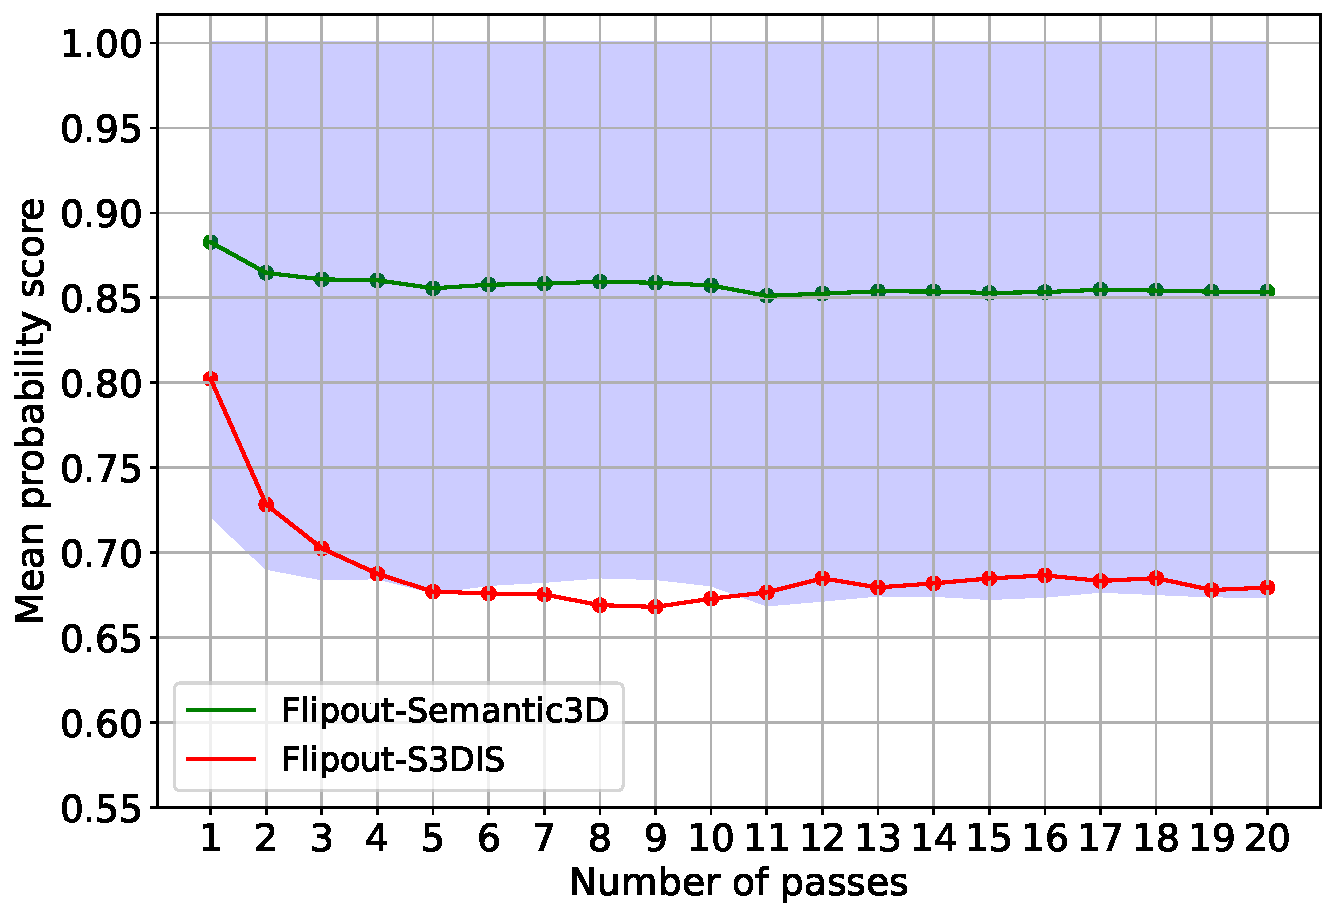
\includegraphics[scale=0.55]{images/Flipout_MSP.pdf}
    %     \caption{}
    %     \label{fig:13_sem3dvs3dis}
    % %\end{subfigure}
    % \end{figure}

    % \begin{figure}[h!]
    %     \centering
    %     \begin{subfigure}{0.98\textwidth}
    %         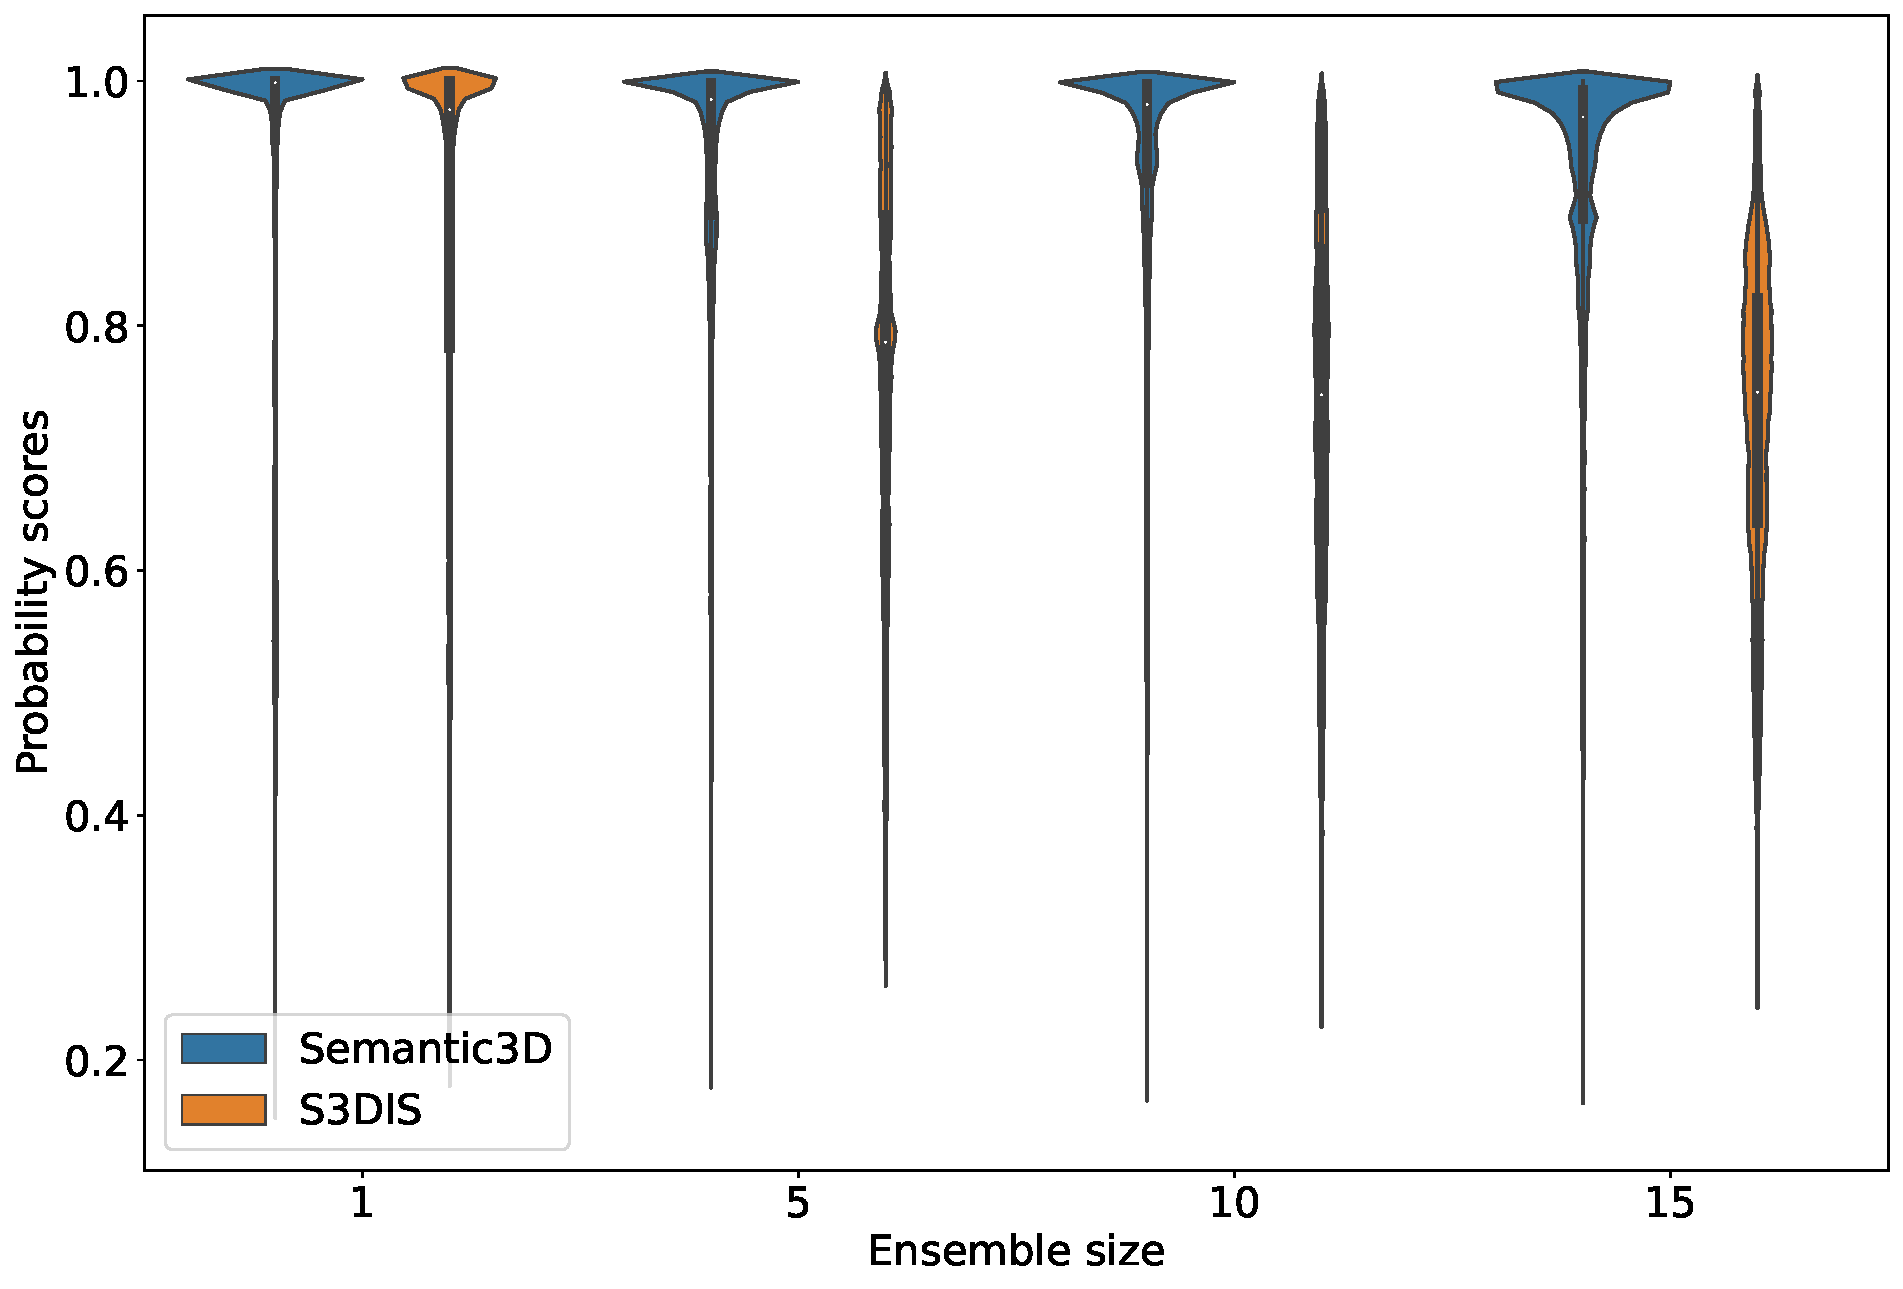
\includegraphics[width=0.98\textwidth, height=0.48\textheight]{images/violin_in_Probability_DE_plot.pdf}
    %     \end{subfigure}
    %     \begin{subfigure}{0.98\textwidth}
    %         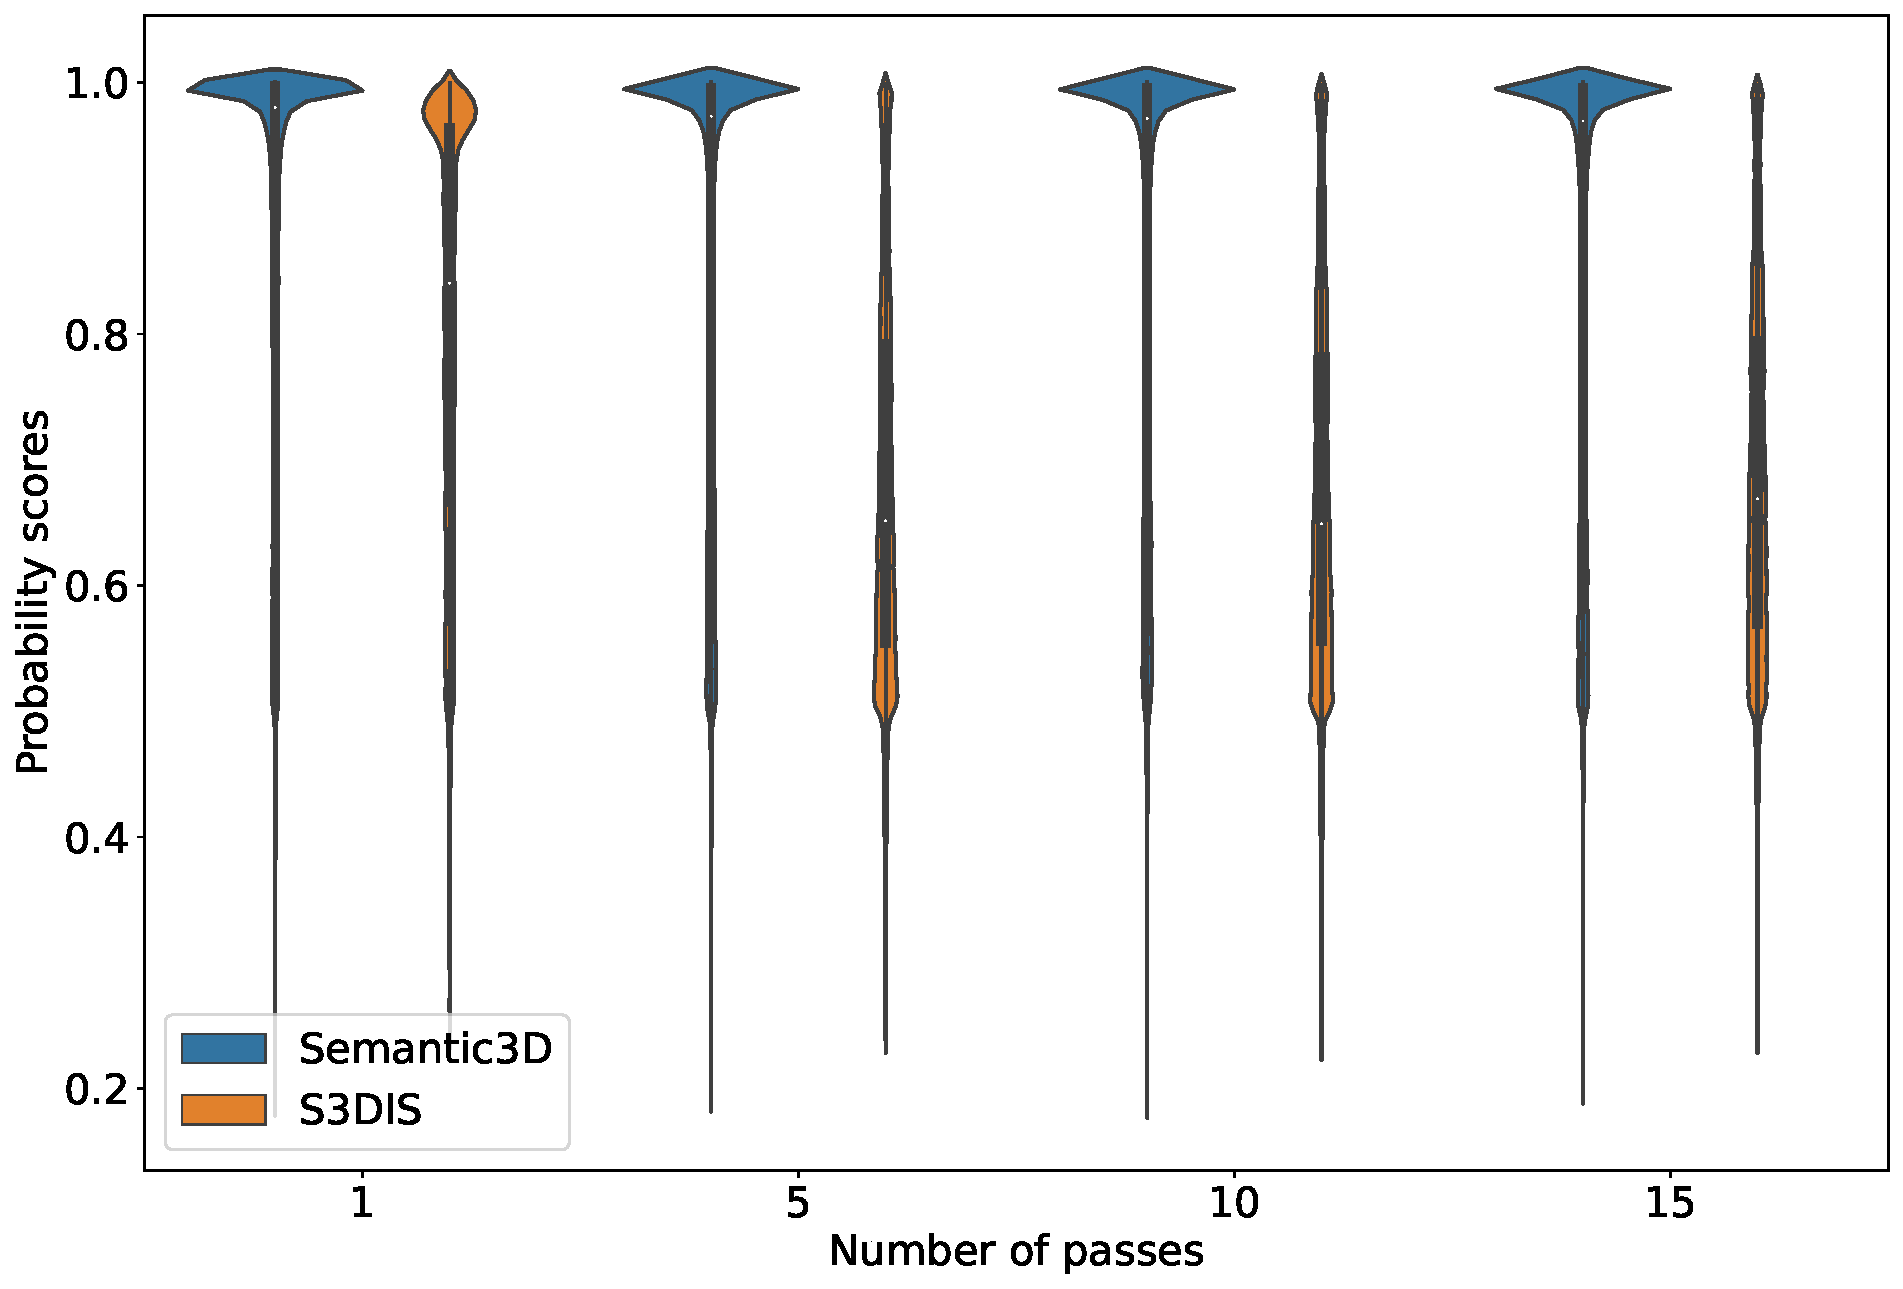
\includegraphics[width=0.98\textwidth, height=0.48\textheight]{images/violin_in_Probability_FOUT_plot.pdf}
    %     \end{subfigure}
    % \end{figure}
    \begin{figure*}[h!]
        \centering
        \begin{tabular}{ccc}
            Ground Truth & Prediction-Deep Ensembles & Probability map-Deep Ensembles \\
            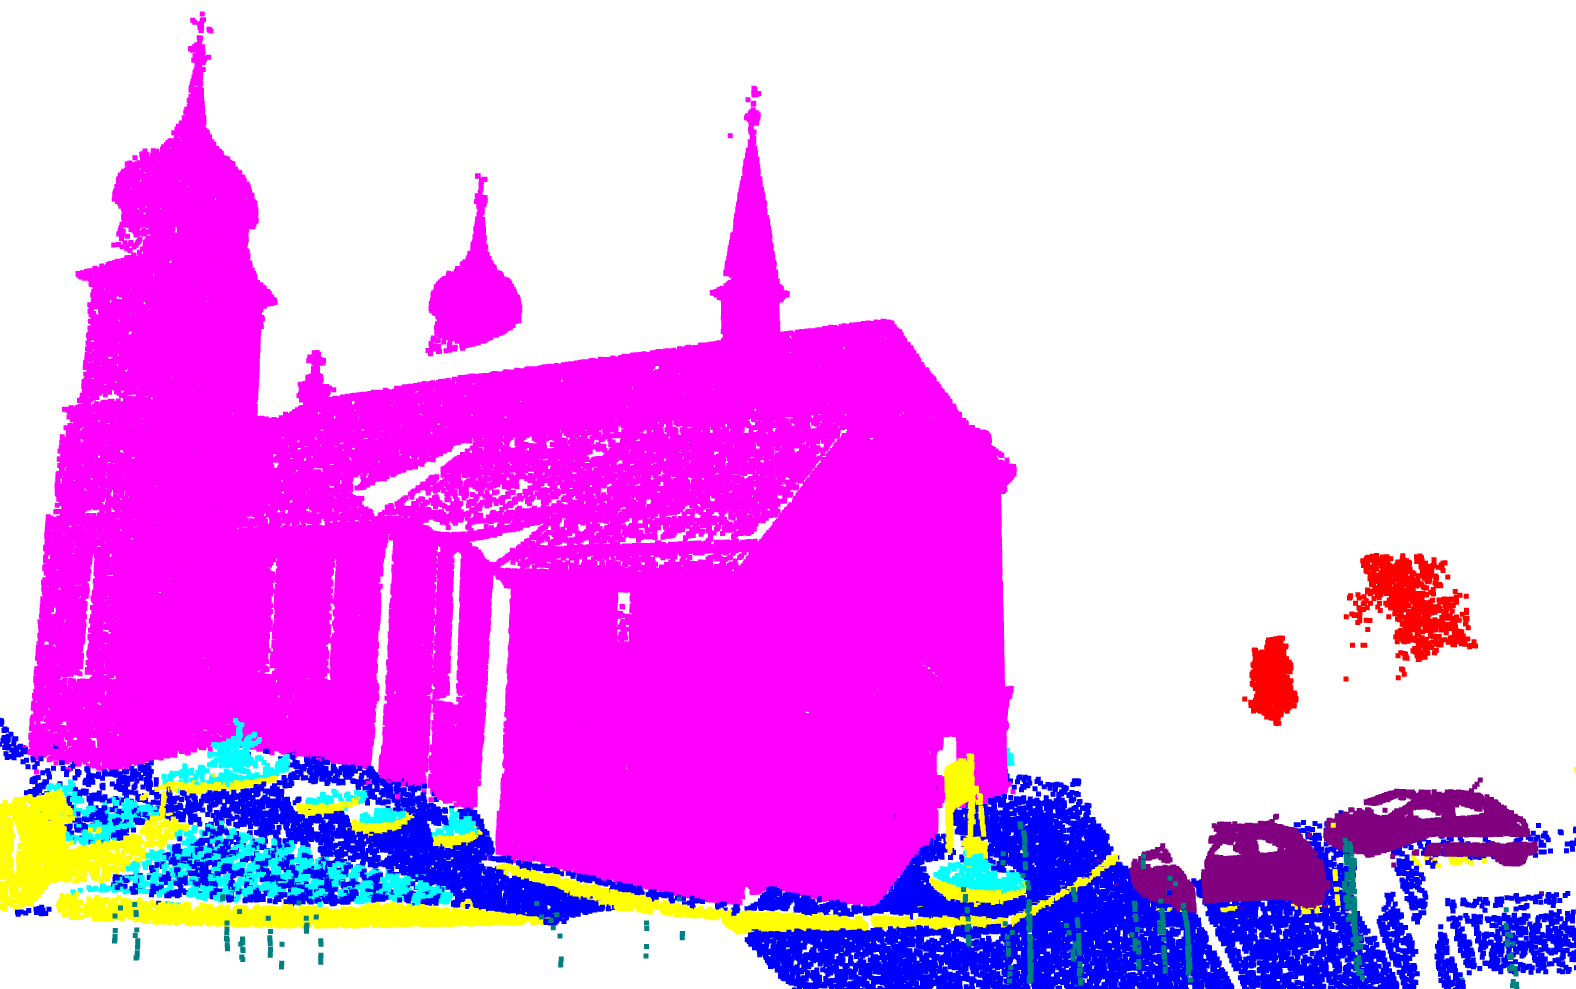
\includegraphics[width=0.33\textwidth, height=0.18\textheight]{images/seg_output/sem3d_seg_output/1_GT.png} &
            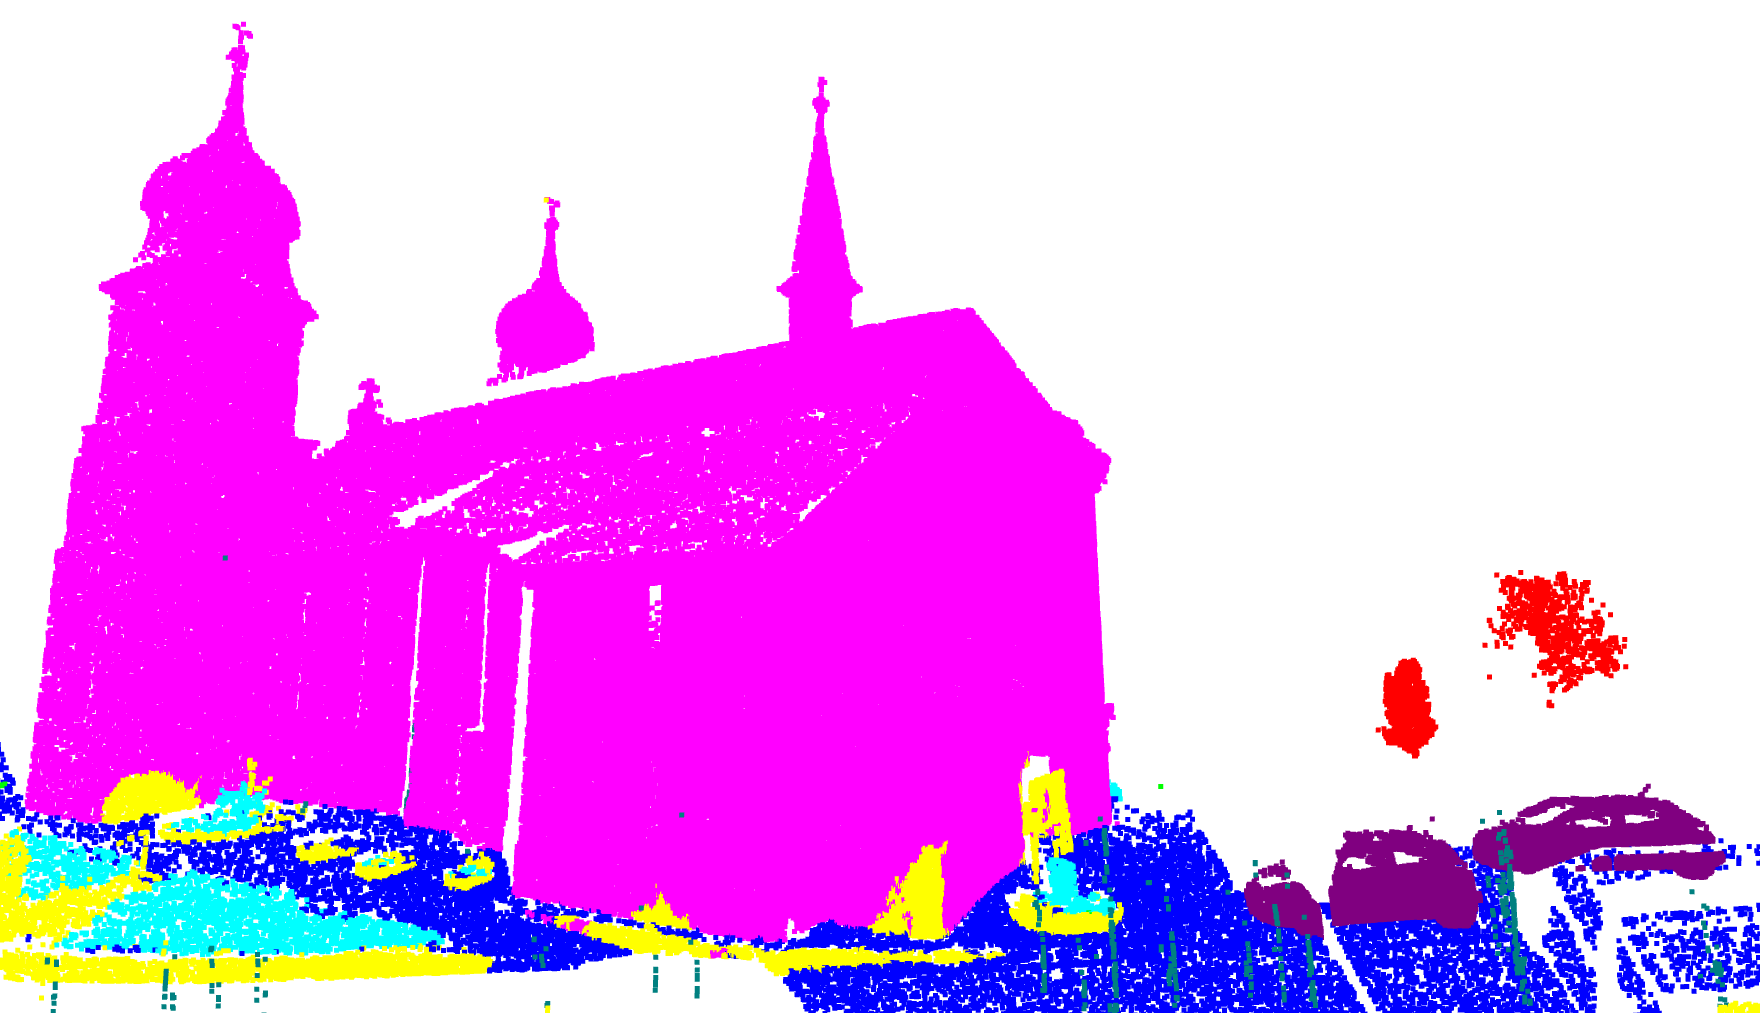
\includegraphics[width=0.33\textwidth, height=0.18\textheight]{images/seg_output/sem3d_seg_output/1_Pred.png}& 
            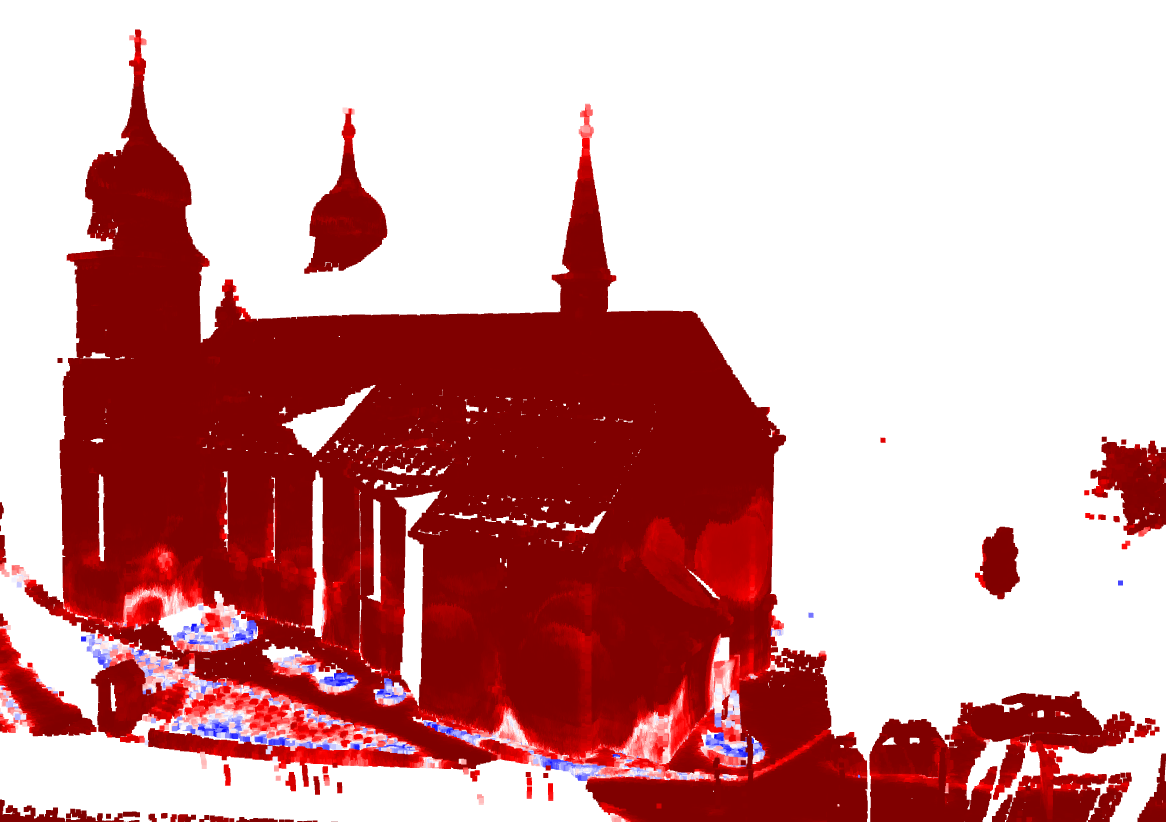
\includegraphics[width=0.33\textwidth, height=0.18\textheight]{images/seg_output/sem3d_seg_output/1_max_prob.png}\\

            \includegraphics[width=0.33\textwidth, height=0.18\textheight]{images/seg_output/sem3d_seg_output/2_GT.png} &
            \includegraphics[width=0.33\textwidth, height=0.18\textheight]{images/seg_output/sem3d_seg_output/2_Pred.png}& 
            \includegraphics[width=0.33\textwidth, height=0.18\textheight]{images/seg_output/sem3d_seg_output/2_max_prob.png}\\

            \includegraphics[width=0.33\textwidth, height=0.18\textheight]{images/seg_output/sem3d_seg_output/3_GT.png} &
            \includegraphics[width=0.33\textwidth, height=0.18\textheight]{images/seg_output/sem3d_seg_output/3_Pred.png}& 
            \includegraphics[width=0.33\textwidth, height=0.18\textheight]{images/seg_output/sem3d_seg_output/3_max_prob.png}\\
        \end{tabular}
        \includegraphics[scale=0.45]{images/prob_legend.pdf}
        \includegraphics[scale=0.65]{images/legend.png}
        \caption{Perpoint probability visualization of the semantic3D dataset.}
        \label{fig:de_sem3d_probmap}
    \end{figure*}

    \begin{figure*}[h!]
        \centering
        \begin{tabular}{ccc}
            Ground Truth & Prediction-Flipout & Probability map-Flipout \\
            \includegraphics[width=0.33\textwidth, height=0.18\textheight]{images/seg_output/sem3d_seg_output/1_GT.png} &
            \includegraphics[width=0.33\textwidth, height=0.18\textheight]{images/seg_output/flipout/sem3d_1.png}& 
            \includegraphics[width=0.33\textwidth, height=0.18\textheight]{images/seg_output/flipout/1_fout_prob.png}\\

            \includegraphics[width=0.33\textwidth, height=0.18\textheight]{images/seg_output/sem3d_seg_output/2_GT.png} &
            \includegraphics[width=0.33\textwidth, height=0.18\textheight]{images/seg_output/flipout/sem3d_2.png}& 
            \includegraphics[width=0.33\textwidth, height=0.18\textheight]{images/seg_output/flipout/2_fout_prob.png}\\

            \includegraphics[width=0.33\textwidth, height=0.18\textheight]{images/seg_output/sem3d_seg_output/3_GT.png} &
            \includegraphics[width=0.33\textwidth, height=0.18\textheight]{images/seg_output/flipout/sem3d_3.png}& 
            \includegraphics[width=0.33\textwidth, height=0.18\textheight]{images/seg_output/flipout/3_fout_prob.png}\\
        \end{tabular}
        \includegraphics[scale=0.45]{images/prob_legend.pdf}
        \includegraphics[scale=0.65]{images/legend.png}
        \caption{Perpoint probability visualization of the semantic3D dataset.}
        \label{fig:fout_sem3d_probmap}
    \end{figure*}

    \begin{figure*}[h!]
        \centering
        \begin{tabular}{cc}
            Prediction-Deep Ensembles & Probability map-Deep Ensembles \\
            \includegraphics[width=0.33\textwidth, height=0.18\textheight]{images/seg_output/s3dis_DE/S3DIS_1_Pred.png}& 
            \includegraphics[width=0.33\textwidth, height=0.18\textheight]{images/seg_output/s3dis_DE/S3DIS_1_prob.png}\\

            \includegraphics[width=0.33\textwidth, height=0.18\textheight]{images/seg_output/s3dis_DE/S3DIS_2_Pred.png}& 
            \includegraphics[width=0.33\textwidth, height=0.18\textheight]{images/seg_output/s3dis_DE/S3DIS_2_prob.png}\\

            \includegraphics[width=0.33\textwidth, height=0.18\textheight]{images/seg_output/s3dis_DE/S3DIS_3_Pred.png}& 
            \includegraphics[width=0.33\textwidth, height=0.18\textheight]{images/seg_output/s3dis_DE/S3DIS_3_prob.png}\\

            \includegraphics[width=0.33\textwidth, height=0.18\textheight]{images/seg_output/s3dis_DE/S3DIS_4_Pred.png}& 
            \includegraphics[width=0.33\textwidth, height=0.18\textheight]{images/seg_output/s3dis_DE/S3DIS_4_prob.png}\\
        \end{tabular}
        \includegraphics[scale=0.45]{images/prob_legend.pdf}
        \includegraphics[scale=0.65]{images/legend.png}
        \caption{Perpoint probability visualization of the S3DIS dataset.}
        \label{fig:de_s3dis_probmap}
    \end{figure*}

    \begin{figure*}[h!]
        \centering
        \begin{tabular}{cc}
            Prediction-Flipout & Probability map-Flipout \\
            \includegraphics[width=0.33\textwidth, height=0.18\textheight]{images/seg_output/s3dis_DE/office_3.png}& 
            \includegraphics[width=0.33\textwidth, height=0.18\textheight]{images/seg_output/s3dis_DE/fout_1.png}\\

            \includegraphics[width=0.33\textwidth, height=0.18\textheight]{images/seg_output/s3dis_DE/ocroom_1.png}& 
            \includegraphics[width=0.33\textwidth, height=0.18\textheight]{images/seg_output/s3dis_DE/fout_2.png}\\

            \includegraphics[width=0.33\textwidth, height=0.18\textheight]{images/seg_output/s3dis_DE/opantry_1.png}& 
            \includegraphics[width=0.33\textwidth, height=0.18\textheight]{images/seg_output/s3dis_DE/fout_3.png}\\

            \includegraphics[width=0.33\textwidth, height=0.18\textheight]{images/seg_output/s3dis_DE/office_42.png}& 
            \includegraphics[width=0.33\textwidth, height=0.18\textheight]{images/seg_output/s3dis_DE/fout_4.png}\\
        \end{tabular}
        \includegraphics[scale=0.45]{images/prob_legend.pdf}
        \includegraphics[scale=0.65]{images/legend.png}
        \caption{Perpoint probability visualization of the S3DIS dataset flipout.}
        \label{fig:fout_s3dis_probmap}
    \end{figure*}

    % \begin{figure}[h!]
    %     \begin{subfigure}{0.495\textwidth}
    %         \includegraphics[scale=0.35]{images/ensemble_probability_sem3dvs3dis_AUROC.pdf}
    %     \end{subfigure}
    %     \begin{subfigure}{0.495\textwidth}
    %         \includegraphics[scale=0.35]{images/flipout_probability_sem3dvs3dis_AUROC.pdf}
    %     \end{subfigure}
    %     \begin{subfigure}{0.98\textwidth}
    %         \centering
    %         \includegraphics[scale=0.35]{images/dropout_probability_sem3dvs3dis_AUROC.pdf}
    %     \end{subfigure}
    %     \caption{Ensmeble Vs Flipout Vs Dropout- Probability scores}
    % \end{figure}
    %%%%%% Entropy (Semantic3D vs S3DIS) %%%%%%
    \FloatBarrier
    \subsection{Entropy}
    \label{sec:ent_sem3dvs3dis}

    Similar to the experiment in Section~[\$], in this experiment, we study the distribution entropy values for ID (Semantic3D) and OOD (S3DIS) datasets.
    Entropy scores are a sum log function of softmax probabilities and detailed discussion in Section~[\$].
    Figure~\ref{fig:ent_ensembles} and Figure~\ref{fig:ent_flipout} depict the mean entropy score and variance plotted as error bars for Deep Ensembles and Flipout methods.    
    Figure~\ref{fig:de_sem3d_entmap} and Figure~\ref{fig:fout_sem3d_entmap} represents the entropy map for the ID dataset generated using Deep Ensembles and Flipout.
    Similarly, Figure~\ref{fig:de_s3dis_entmap} and Figure~\ref{fig:fout_s3dis_entmap} represents the entropy map for the OOD dataset.

    From Figure~\ref{fig:ent_ensembles} and Figure~\ref{fig:ent_flipout}, we observe the entropy for the ID dataset is lower because the softmax values are not highly distributed across all the classes.
    Whereas in the case OOD dataset, the softmax probabilities are highly distributed across all the classes, so we observe a higher entropy score.
    Similar to the probability score, we also observe a decrement in the variance of entropy score until the ensemble size of 13 and then stabilizes out.
    Also, we infer that there is a lesser overlap between the error bars of OOD and ID datasets in the case of Deep Ensembles than the Flipout.
    So in both cases of MSP and entropy, we expect the Deep Ensembles to detect OOD objects better than the Flipout.

    On careful observation of Figure~\ref{fig:de_sem3d_entmap} and Figure~\ref{fig:fout_sem3d_entmap}, we infer that overall entropy map is more bluish in shade representing the lower entropy scores.
    A higher entropy (yellow) is observed at the points of misclassifications and along the edges (similar to the case of probability map in Figures~\ref{fig:de_sem3d_probmap}, \ref{fig:fout_sem3d_probmap}).
    An example of misclassified points having higher entropy is observed in Figure~\ref{fig:fout_sem3d_entmap}, where the misclassified top of the church is greener on the entropy map compared to the rest of the church building.
    Visually observation of entropy maps for the OOD dataset in Figure~\ref{fig:de_s3dis_entmap} and Figure~\ref{fig:fout_s3dis_entmap} reveals the colours to be at the higher end of the entropy scale resulting in a more yellowish shade in the case of both Flipout and Deep Ensembles.

    \begin{figure}[!ht]
        \centering
        \begin{subfigure}{0.98\textwidth}
        \includegraphics[scale=0.6]{images/MSP/Ensembles_ENT_cnc.pdf}
        \caption{Entropy deep ensembles, (mistake in x axis)}
        \label{fig:ent_ensembles}
        \end{subfigure}
        \begin{subfigure}{0.98\textwidth}
        \includegraphics[scale=0.6]{images/MSP/Flipout_ENT_cnc.pdf}
        \caption{Entropy flipout}
        \label{fig:ent_flipout}
        \end{subfigure}
    \end{figure}
    \begin{figure*}[h!]
        \begin{tabular}{ccc}
            Ground Truth & Prediction-Deep Ensembles & Entropy map-Deep Ensembles \\
            \includegraphics[width=0.33\textwidth, height=0.18\textheight]{images/seg_output/sem3d_seg_output/1_GT.png} &
            \includegraphics[width=0.33\textwidth, height=0.18\textheight]{images/seg_output/sem3d_seg_output/1_Pred.png}& 
            \includegraphics[width=0.33\textwidth, height=0.18\textheight]{images/seg_output/sem3d_seg_output/ent_de_1.png}\\

            \includegraphics[width=0.33\textwidth, height=0.18\textheight]{images/seg_output/sem3d_seg_output/2_GT.png} &
            \includegraphics[width=0.33\textwidth, height=0.18\textheight]{images/seg_output/sem3d_seg_output/2_Pred.png}& 
            \includegraphics[width=0.33\textwidth, height=0.18\textheight]{images/seg_output/sem3d_seg_output/ent_de_2.png}\\

            \includegraphics[width=0.33\textwidth, height=0.18\textheight]{images/seg_output/sem3d_seg_output/3_GT.png} &
            \includegraphics[width=0.33\textwidth, height=0.18\textheight]{images/seg_output/sem3d_seg_output/3_Pred.png}& 
            \includegraphics[width=0.33\textwidth, height=0.18\textheight]{images/seg_output/sem3d_seg_output/ent_de_3.png}\\
        \end{tabular}
        \includegraphics[scale=0.45]{images/prob_legend.pdf}
        \includegraphics[scale=0.65]{images/legend.png}
        \caption{Perpoint entropy visualization of the semantic3D dataset-Ensembles. (Chnage the scale)}
        \label{fig:de_sem3d_entmap}
    \end{figure*}

    \begin{figure*}[h!]
        \centering
        \begin{tabular}{ccc}
            Ground Truth & Prediction-Flipout & Entropy map-Flipout \\
            \includegraphics[width=0.33\textwidth, height=0.18\textheight]{images/seg_output/sem3d_seg_output/1_GT.png} &
            \includegraphics[width=0.33\textwidth, height=0.18\textheight]{images/seg_output/flipout/sem3d_1.png}& 
            \includegraphics[width=0.33\textwidth, height=0.18\textheight]{images/seg_output/sem3d_seg_output/ent_fout_1.png}\\

            \includegraphics[width=0.33\textwidth, height=0.18\textheight]{images/seg_output/sem3d_seg_output/2_GT.png} &
            \includegraphics[width=0.33\textwidth, height=0.18\textheight]{images/seg_output/flipout/sem3d_2.png}& 
            \includegraphics[width=0.33\textwidth, height=0.18\textheight]{images/seg_output/sem3d_seg_output/ent_fout_2.png}\\

            \includegraphics[width=0.33\textwidth, height=0.18\textheight]{images/seg_output/sem3d_seg_output/3_GT.png} &
            \includegraphics[width=0.33\textwidth, height=0.18\textheight]{images/seg_output/flipout/sem3d_3.png}& 
            \includegraphics[width=0.33\textwidth, height=0.18\textheight]{images/seg_output/sem3d_seg_output/ent_fout_3.png}\\
        \end{tabular}
        \includegraphics[scale=0.45]{images/prob_legend.pdf}
        \includegraphics[scale=0.65]{images/legend.png}
        \caption{Perpoint entropy visualization of the semantic3D dataset.}
        \label{fig:fout_sem3d_entmap}
    \end{figure*}
    \begin{figure*}[h!]
        \centering
        \begin{tabular}{cc}
            Prediction-Deep Ensembles & Entropy map-Deep Ensembles \\
            \includegraphics[width=0.33\textwidth, height=0.18\textheight]{images/seg_output/s3dis_DE/S3DIS_1_Pred.png}& 
            \includegraphics[width=0.33\textwidth, height=0.18\textheight]{images/seg_output/flipout/ent_de_s3dis_3.png}\\

            \includegraphics[width=0.33\textwidth, height=0.18\textheight]{images/seg_output/s3dis_DE/S3DIS_2_Pred.png}& 
            \includegraphics[width=0.33\textwidth, height=0.18\textheight]{images/seg_output/flipout/ent_de_s3dis_1.png}\\

            \includegraphics[width=0.33\textwidth, height=0.18\textheight]{images/seg_output/s3dis_DE/S3DIS_3_Pred.png}& 
            \includegraphics[width=0.33\textwidth, height=0.18\textheight]{images/seg_output/flipout/ent_de_s3dis_2.png}\\

            \includegraphics[width=0.33\textwidth, height=0.18\textheight]{images/seg_output/s3dis_DE/S3DIS_4_Pred.png}& 
            \includegraphics[width=0.33\textwidth, height=0.18\textheight]{images/seg_output/flipout/ent_de_s3dis_4.png}\\
        \end{tabular}
        \includegraphics[scale=0.45]{images/prob_legend.pdf}
        \includegraphics[scale=0.65]{images/legend.png}
        \caption{Perpoint entropy visualization of the S3DIS dataset.}
        \label{fig:de_s3dis_entmap}
    \end{figure*}
    \begin{figure*}[h!]
        \centering
        \begin{tabular}{cc}
            Prediction-Flipout & Entropy map-Flipout \\
            \includegraphics[width=0.33\textwidth, height=0.18\textheight]{images/seg_output/s3dis_DE/office_3.png}& 
            \includegraphics[width=0.33\textwidth, height=0.18\textheight]{images/seg_output/flipout/ent_fout_s3dis_3.png}\\

            \includegraphics[width=0.33\textwidth, height=0.18\textheight]{images/seg_output/s3dis_DE/ocroom_1.png}& 
            \includegraphics[width=0.33\textwidth, height=0.18\textheight]{images/seg_output/flipout/ent_fout_s3dis_1.png}\\

            \includegraphics[width=0.33\textwidth, height=0.18\textheight]{images/seg_output/s3dis_DE/opantry_1.png}& 
            \includegraphics[width=0.33\textwidth, height=0.18\textheight]{images/seg_output/flipout/ent_fout_s3dis_2.png}\\

            \includegraphics[width=0.33\textwidth, height=0.18\textheight]{images/seg_output/s3dis_DE/office_42.png}& 
            \includegraphics[width=0.33\textwidth, height=0.18\textheight]{images/seg_output/flipout/ent_fout_s3dis_4.png}\\
        \end{tabular}
        \includegraphics[scale=0.45]{images/prob_legend.pdf}
        \includegraphics[scale=0.65]{images/legend.png}
        \caption{Perpoint entropy visualization of the S3DIS dataset flipout.}
        \label{fig:fout_s3dis_entmap}
    \end{figure*}
    \FloatBarrier
    \section{OOD detection evaluation - Semantic3D vs S3DIS}
    \begin{table}[h!]
        \centering
        \begin{tabular}{cccc}
        \hline
        Ensemble size/ \#passes & Method               &  \multicolumn{2}{c}{AUROC}          \\ \hline
                                &                      &  MSP              & Entropy         \\ \hline
        \multirow{3}{*}{1}      & Dropout              & 0.53311          & 0.53041          \\
                                & Flipout              & \textbf{0.69988} & \textbf{0.69368} \\
                                & Deep Ensembles       & 0.62020          & 0.62529          \\ \hline
        \multirow{3}{*}{5}      & Dropout              & 0.58439          & 0.57821          \\
                                & Flipout              & 0.77885          & 0.76934          \\
                                & Deep Ensembles       & \textbf{0.84013} & \textbf{0.83665} \\ \hline
        \multirow{3}{*}{10}     & Dropout              & 0.60168          & 0.59925          \\
                                & Flipout              & 0.78728          & 0.78327          \\
                                & Deep Ensembles       & \textbf{0.87929} & \textbf{0.87541} \\ \hline
        \multirow{3}{*}{15}     & Dropout              & 0.59773          & 0.59557          \\
                                & Flipout              & 0.7667           & 0.76741          \\
                                & Deep Ensembles       & \textbf{0.88486} & \textbf{0.88246} \\ \hline
        \multirow{3}{*}{20}     & Dropout              & 0.59766          & 0.59661          \\
                                & Flipout              & 0.77331          & 0.77237          \\
                                & Deep Ensembles       & \textbf{0.89338} & \textbf{0.89052} \\ \hline
        \end{tabular}
        \caption{AUROC scores}
    \end{table}
    
        \begin{figure*}[h!]
            \centering
            \begin{tabular}{cc}
                % Prediction-Deep Ensembles & 
                Probability map-Deep Ensembles & OOD map-Deep Ensembles \\
                % \includegraphics[width=0.33\textwidth, height=0.18\textheight]{images/ood_imgs/de_sem3d/de_class_prob_1.png} &
                \includegraphics[width=0.33\textwidth, height=0.18\textheight]{images/ood_imgs/de_sem3d/de_prob_10_1.png}& 
                \includegraphics[width=0.33\textwidth, height=0.18\textheight]{images/ood_imgs/de_sem3d/de_ood_auroc_1.png}\\
    
                % \includegraphics[width=0.33\textwidth, height=0.18\textheight]{images/ood_imgs/de_sem3d/de_class_prob_2.png} &
                \includegraphics[width=0.33\textwidth, height=0.18\textheight]{images/ood_imgs/de_sem3d/de_prob_10_2.png}& 
                \includegraphics[width=0.33\textwidth, height=0.18\textheight]{images/ood_imgs/de_sem3d/de_ood_auroc_2.png}\\
    
                % \includegraphics[width=0.33\textwidth, height=0.18\textheight]{images/ood_imgs/de_sem3d/de_class_prob_3.png} &
                \includegraphics[width=0.33\textwidth, height=0.18\textheight]{images/ood_imgs/de_sem3d/de_prob_10_3.png}& 
                \includegraphics[width=0.33\textwidth, height=0.18\textheight]{images/ood_imgs/de_sem3d/de_ood_auroc_3.png}\\
            \end{tabular}
            \includegraphics[scale=0.45]{images/prob_legend.pdf}
            % \includegraphics[scale=0.65]{images/legend.png}
            \caption{OOD point visualization of the semantic3D dataset Deep Ensembles-size 10.}
            \label{fig:de_ood_auroc_sem3d_prob}
        \end{figure*}
        \begin{figure*}[h!]
            \centering
            \begin{tabular}{cc}
                % Prediction-Flipout & 
                Probability map-Flipout & OOD map-Flipout \\
                % \includegraphics[width=0.33\textwidth, height=0.18\textheight]{images/ood_imgs/fout_sem3d/fout_1.png} &
                \includegraphics[width=0.33\textwidth, height=0.18\textheight]{images/ood_imgs/fout_sem3d/fout_prob_1.png}& 
                \includegraphics[width=0.33\textwidth, height=0.18\textheight]{images/ood_imgs/fout_sem3d/fout_ood_auroc_1.png}\\

                % \includegraphics[width=0.33\textwidth, height=0.18\textheight]{images/ood_imgs/fout_sem3d/fout_2.png} &
                \includegraphics[width=0.33\textwidth, height=0.18\textheight]{images/ood_imgs/fout_sem3d/fout_prob_2.png}& 
                \includegraphics[width=0.33\textwidth, height=0.18\textheight]{images/ood_imgs/fout_sem3d/fout_ood_auroc_2.png}\\
    
                % \includegraphics[width=0.33\textwidth, height=0.18\textheight]{images/ood_imgs/fout_sem3d/fout_3.png} &
                \includegraphics[width=0.33\textwidth, height=0.18\textheight]{images/ood_imgs/fout_sem3d/fout_prob_3.png}& 
                \includegraphics[width=0.33\textwidth, height=0.18\textheight]{images/ood_imgs/fout_sem3d/fout_ood_auroc_3.png}\\
            \end{tabular}
            \includegraphics[scale=0.45]{images/prob_legend.pdf}
            % \includegraphics[scale=0.65]{images/legend.png}
            \caption{OOD point visualization of the semantic3D dataset Deep Ensembles-size 10.}
            \label{fig:fout_ood_auroc_sem3d_prob}
        \end{figure*}
        \begin{figure*}[h!]
            \centering
            \begin{tabular}{cc}
                Entropy map-Deep Ensembles & OOD map-Deep Ensembles \\
                % \includegraphics[width=0.33\textwidth, height=0.18\textheight]{images/ood_imgs/de_sem3d/de_class_prob_1.png} &
                \includegraphics[width=0.33\textwidth, height=0.18\textheight]{images/ood_imgs/de_sem3d/de_ent_10_1.png}& 
                \includegraphics[width=0.33\textwidth, height=0.18\textheight]{images/ood_imgs/de_sem3d/de_ent_ood_auroc_1.png}\\
    
                % \includegraphics[width=0.33\textwidth, height=0.18\textheight]{images/ood_imgs/de_sem3d/de_class_prob_2.png} &
                \includegraphics[width=0.33\textwidth, height=0.18\textheight]{images/ood_imgs/de_sem3d/de_ent_10_2.png}& 
                \includegraphics[width=0.33\textwidth, height=0.18\textheight]{images/ood_imgs/de_sem3d/de_ent_ood_auroc_2.png}\\
    
                % \includegraphics[width=0.33\textwidth, height=0.18\textheight]{images/ood_imgs/de_sem3d/de_class_prob_3.png} &
                \includegraphics[width=0.33\textwidth, height=0.18\textheight]{images/ood_imgs/de_sem3d/de_ent_10_3.png}& 
                \includegraphics[width=0.33\textwidth, height=0.18\textheight]{images/ood_imgs/de_sem3d/de_ent_ood_auroc_3.png}\\
            \end{tabular}
            \includegraphics[scale=0.45]{images/prob_legend.pdf}
            % \includegraphics[scale=0.65]{images/legend.png}
            \caption{OOD point visualization of the semantic3D dataset Deep Ensembles-size 10.}
            \label{fig:de_ood_auroc_sem3d_ent}
        \end{figure*}
        \begin{figure*}[h!]
            \centering
            % \begin{tabular}{ccc}
            \begin{tabular}{cc}
                % Prediction-Flipout & Entropy map-Flipout & OOD map-Flipout \\
                Entropy map-Flipout & OOD map-Flipout \\
                % \includegraphics[width=0.33\textwidth, height=0.18\textheight]{images/ood_imgs/fout_sem3d/fout_1.png} &
                \includegraphics[width=0.33\textwidth, height=0.18\textheight]{images/ood_imgs/fout_sem3d/fout_ent_1.png}& 
                \includegraphics[width=0.33\textwidth, height=0.18\textheight]{images/ood_imgs/fout_sem3d/fout_ent_ood_auroc_1.png}\\

                % \includegraphics[width=0.33\textwidth, height=0.18\textheight]{images/ood_imgs/fout_sem3d/fout_2.png} &
                \includegraphics[width=0.33\textwidth, height=0.18\textheight]{images/ood_imgs/fout_sem3d/fout_ent_2.png}& 
                \includegraphics[width=0.33\textwidth, height=0.18\textheight]{images/ood_imgs/fout_sem3d/fout_ent_ood_auroc_2.png}\\
    
                % \includegraphics[width=0.33\textwidth, height=0.18\textheight]{images/ood_imgs/fout_sem3d/fout_3.png} &
                \includegraphics[width=0.33\textwidth, height=0.18\textheight]{images/ood_imgs/fout_sem3d/fout_ent_3.png}& 
                \includegraphics[width=0.33\textwidth, height=0.18\textheight]{images/ood_imgs/fout_sem3d/fout_ent_ood_auroc_3.png}\\
            \end{tabular}
            \includegraphics[scale=0.45]{images/prob_legend.pdf}
            % \includegraphics[scale=0.65]{images/legend.png}
            \caption{OOD point visualization of the semantic3D dataset Deep Ensembles-size 10.}
            \label{fig:fout_ood_auroc_sem3d_ent}
        \end{figure*}

        \begin{figure*}[h!]
            \centering
            \begin{tabular}{cc}
                Probability map-Deep Ensembles & OOD map-Deep Ensembles \\
                \includegraphics[width=0.33\textwidth, height=0.18\textheight]{images/ood_imgs/de_s3dis/ofc_3_de_prob.png}& 
                \includegraphics[width=0.33\textwidth, height=0.18\textheight]{images/ood_imgs/de_s3dis/de_prob_2.png}\\
    
                \includegraphics[width=0.33\textwidth, height=0.18\textheight]{images/ood_imgs/de_s3dis/cf1_de_prob.png}& 
                \includegraphics[width=0.33\textwidth, height=0.18\textheight]{images/ood_imgs/de_s3dis/de_prob_4.png}\\
    
                \includegraphics[width=0.33\textwidth, height=0.18\textheight]{images/ood_imgs/de_s3dis/pnt_1_de_prob.png}& 
                \includegraphics[width=0.33\textwidth, height=0.18\textheight]{images/ood_imgs/de_s3dis/de_prob_3.png}\\
    
                \includegraphics[width=0.33\textwidth, height=0.18\textheight]{images/ood_imgs/de_s3dis/ofc_42_de_prob.png}& 
                \includegraphics[width=0.33\textwidth, height=0.18\textheight]{images/ood_imgs/de_s3dis/de_prob_1.png}\\
            \end{tabular}
            \includegraphics[scale=0.45]{images/prob_legend.pdf}
            % \includegraphics[scale=0.65]{images/legend.png}
            \caption{OOD visualization of the S3DIS dataset Deep Ensembles.}
            \label{fig:de_s3dis_oodmap_prob}
        \end{figure*}
        \begin{figure*}[h!]
            \centering
            \begin{tabular}{cc}
                Probability map-Flipout & OOD map-Flipout \\
                \includegraphics[width=0.33\textwidth, height=0.18\textheight]{images/ood_imgs/fout_s3dis/ofc_3_fout_prob.png}& 
                \includegraphics[width=0.33\textwidth, height=0.18\textheight]{images/ood_imgs/fout_s3dis/fout_prob_2.png}\\
    
                \includegraphics[width=0.33\textwidth, height=0.18\textheight]{images/ood_imgs/fout_s3dis/cf1_fout_prob.png}& 
                \includegraphics[width=0.33\textwidth, height=0.18\textheight]{images/ood_imgs/fout_s3dis/fout_prob_4.png}\\
    
                \includegraphics[width=0.33\textwidth, height=0.18\textheight]{images/ood_imgs/fout_s3dis/pnt_1_fout_prob.png}& 
                \includegraphics[width=0.33\textwidth, height=0.18\textheight]{images/ood_imgs/fout_s3dis/fout_prob_3.png}\\
    
                \includegraphics[width=0.33\textwidth, height=0.18\textheight]{images/ood_imgs/fout_s3dis/ofc_42_fout_prob.png}& 
                \includegraphics[width=0.33\textwidth, height=0.18\textheight]{images/ood_imgs/fout_s3dis/fout_prob_1.png}\\
            \end{tabular}
            \includegraphics[scale=0.45]{images/prob_legend.pdf}
            % \includegraphics[scale=0.65]{images/legend.png}
            \caption{OOD visualization of the S3DIS dataset Flipout.}
            \label{fig:fout_s3dis_oodmap_prob}
        \end{figure*}


        \begin{figure*}[h!]
            \centering
            \begin{tabular}{cc}
                Entropy map-Deep Ensembles & OOD map-Deep Ensembles \\
                \includegraphics[width=0.33\textwidth, height=0.18\textheight]{images/ood_imgs/de_s3dis/ofc_3_de_ent.png}& 
                \includegraphics[width=0.33\textwidth, height=0.18\textheight]{images/ood_imgs/de_s3dis/de_ent_2.png}\\
    
                \includegraphics[width=0.33\textwidth, height=0.18\textheight]{images/ood_imgs/de_s3dis/cf1_de_ent.png}& 
                \includegraphics[width=0.33\textwidth, height=0.18\textheight]{images/ood_imgs/de_s3dis/de_ent_4.png}\\
    
                \includegraphics[width=0.33\textwidth, height=0.18\textheight]{images/ood_imgs/de_s3dis/pnt_1_de_ent.png}& 
                \includegraphics[width=0.33\textwidth, height=0.18\textheight]{images/ood_imgs/de_s3dis/de_ent_3.png}\\
    
                \includegraphics[width=0.33\textwidth, height=0.18\textheight]{images/ood_imgs/de_s3dis/ofc_42_de_ent.png}& 
                \includegraphics[width=0.33\textwidth, height=0.18\textheight]{images/ood_imgs/de_s3dis/de_ent_1.png}\\
            \end{tabular}
            \includegraphics[scale=0.45]{images/prob_legend.pdf}
            % \includegraphics[scale=0.65]{images/legend.png}
            \caption{OOD visualization of the S3DIS dataset Deep Ensembles.}
            \label{fig:de_s3dis_oodmap_ent}
        \end{figure*}
        \begin{figure*}[h!]
            \centering
            \begin{tabular}{cc}
                Entropy map-Flipout & OOD map-Flipout \\
                \includegraphics[width=0.33\textwidth, height=0.18\textheight]{images/ood_imgs/fout_s3dis/ofc_3_fout_ent.png}& 
                \includegraphics[width=0.33\textwidth, height=0.18\textheight]{images/ood_imgs/fout_s3dis/fout_ent_2.png}\\
    
                \includegraphics[width=0.33\textwidth, height=0.18\textheight]{images/ood_imgs/fout_s3dis/cf1_fout_ent.png}& 
                \includegraphics[width=0.33\textwidth, height=0.18\textheight]{images/ood_imgs/fout_s3dis/fout_ent_4.png}\\
    
                \includegraphics[width=0.33\textwidth, height=0.18\textheight]{images/ood_imgs/fout_s3dis/pnt_1_fout_ent.png}& 
                \includegraphics[width=0.33\textwidth, height=0.18\textheight]{images/ood_imgs/fout_s3dis/fout_ent_3.png}\\
    
                \includegraphics[width=0.33\textwidth, height=0.18\textheight]{images/ood_imgs/fout_s3dis/ofc_42_fout_ent.png}& 
                \includegraphics[width=0.33\textwidth, height=0.18\textheight]{images/ood_imgs/fout_s3dis/fout_ent_1.png}\\
            \end{tabular}
            \includegraphics[scale=0.45]{images/prob_legend.pdf}
            % \includegraphics[scale=0.65]{images/legend.png}
            \caption{OOD visualization of the S3DIS dataset Deep Ensembles.}
            \label{fig:fout_s3dis_oodmap_ent}
        \end{figure*}
        \FloatBarrier


    \section{OOD Benchmark - Semantic3D vs Semantic3D without color}
    \subsection{Deep ensembles}
    % \begin{table}[h!]
    %     \resizebox{\textwidth}{!}{%
    %     \begin{tabular}{c|c|cccccccc|c}
    %     %\textbf{\#Ensembles} & \textbf{MeanIOU} & \textbf{Accuracy} & \textbf{Manmadeterrain} & \textbf{Naturalterrain} & \textbf{Highvegetation} & \textbf{Lowvegetation} & \textbf{Buildings} & \textbf{Hardscapes} & \textbf{Scanningartifacts} & \textbf{Cars} \\ \hline
    %     & & \multicolumn{7}{c}{\textbf{IoU per class}} & \\ \hline
    %     \textbf{\#Ensembles} & \textbf{MeanIOU} & \textbf{C1} & \textbf{C2} & \textbf{C3} & \textbf{C4} & \textbf{C5} & \textbf{C6} & \textbf{C7} & \textbf{C8} & \textbf{Accuracy} \\ \hline
    %     1& 68.19& 94.55& 81.19& 84.67& 29.43& 81.37& 18.85& 64.74& 90.74& 88.78 \\
    %     5& 69.51& 94.73& 81.92& 84.42& 28.05& \textbf{86.41}& 28.50& 61.03& 91.03& 90.04 \\
    %     10& 69.97& 95.25& 83.73& 86.63& 30.36& 84.13& 18.60& \textbf{66.01}& 92.61& 89.94 \\
    %     15& 70.32& 95.27& 83.54& \textbf{88.22}& \textbf{32.19}& 84.82& 26.17& 61.67& 90.75& \textbf{90.57} \\
    %     20& \textbf{70.80}& \textbf{95.55}& \textbf{84.11}& 86.65& 29.60& 85.41& \textbf{29.58}& 62.47& \textbf{93.06}& 90.56 \\
    %     \end{tabular}%
    %     }
    %     \caption{Illustration of performance of RandLA-Net on Semantic3D over number of ensembles. meanIOU and IOU per class and overall accuracy are represented here.
    %     C1 to C8 are the classes of Semantic3D which are Manmadeterrain, Naturalterrain, Highvegetation, Lowvegetation, Buildings, Hardscapes, Scanningartifacts, and Cars.}
    % \end{table}

    \begin{table}[h!]
        \resizebox{\textwidth}{!}{%
        \begin{tabular}{c|c|cccccccc|c}
        %\textbf{\#Ensembles} & \textbf{MeanIOU} & \textbf{Accuracy} & \textbf{Manmadeterrain} & \textbf{Naturalterrain} & \textbf{Highvegetation} & \textbf{Lowvegetation} & \textbf{Buildings} & \textbf{Hardscapes} & \textbf{Scanningartifacts} & \textbf{Cars} \\ \hline
        & & \multicolumn{7}{c}{\textbf{IoU per class}} & \\ \hline
        \textbf{Ensemble size} & \textbf{MeanIOU} & \textbf{C1} & \textbf{C2} & \textbf{C3} & \textbf{C4} & \textbf{C5} & \textbf{C6} & \textbf{C7} & \textbf{C8} & \textbf{Accuracy} \\ \hline
        1& 47.96&78.67&7.21&78.63&23.54&85.37&15.48&45.96&48.83&80.26\\
        5& 49.66&80.68&4.49&79.06&26.87&84.87&16.64&48.79&55.85&81.62\\
        10& 50.39&80.86&5.17&78.97&27.25&84.52&16.75&48.02&61.54&81.65\\
        15& 50.33&81.02&5.04&77.25&27.52&83.18&16.53&47.81&64.25&81.25\\
        20& 50.24&81.01&5.15&77.20&27.3&83.60&17.07&47.74&62.83&81.29\\
        \end{tabular}%
        }
        \caption{Illustration of performance of RandLA-Net on Semantic3D wihtout color over number of ensembles. meanIOU and IOU per class and overall accuracy are represented here.
        C1 to C8 are the classes of Semantic3D which are Manmadeterrain, Naturalterrain, Highvegetation, Lowvegetation, Buildings, Hardscapes, Scanningartifacts, and Cars.}
    \end{table}
    \begin{figure*}[h!]
        \centering
        \begin{tabular}{cc}
            Prediction(Semantic3D) & Prediction(Semantic3D without color)\\
            \includegraphics[width=0.33\textwidth, height=0.18\textheight]{images/ood_imgs/de_sem3d/de_class_prob_1.png}&
            \includegraphics[width=0.33\textwidth, height=0.18\textheight]{images/sem3d_of/de_sem3d_of_1.png}\\

            \includegraphics[width=0.33\textwidth, height=0.18\textheight]{images/ood_imgs/de_sem3d/de_class_prob_2.png}&
            \includegraphics[width=0.33\textwidth, height=0.18\textheight]{images/sem3d_of/de_sem3d_of_2.png}\\

            \includegraphics[width=0.33\textwidth, height=0.18\textheight]{images/ood_imgs/de_sem3d/de_class_prob_3.png}&
            \includegraphics[width=0.33\textwidth, height=0.18\textheight]{images/sem3d_of/de_sem3d_of_3.png}\\
        \end{tabular}
        \includegraphics[scale=0.65]{images/legend.png}
        \caption{Output predictions of the RandLA-Net over the Semantic3D dataset and Semantic3D without color
         dataset  (10 number of passes) \textcolor{red}{Legend spelling mistake}.}
        \label{fig:deepensemble_vis_sem3d_OF}
    \end{figure*}
    
    \FloatBarrier
    
    \subsection{Flipout}

    \begin{figure*}[h!]
        \centering
        \begin{tabular}{cc}
            Prediction(Semantic3D) & Prediction(Semantic3D without color) \\
            \includegraphics[width=0.33\textwidth, height=0.18\textheight]{images/ood_imgs/fout_sem3d/fout_1.png}&
            \includegraphics[width=0.33\textwidth, height=0.18\textheight]{images/sem3d_of/fout_sem3d_of_1.png}\\

            \includegraphics[width=0.33\textwidth, height=0.18\textheight]{images/ood_imgs/fout_sem3d/fout_2.png}&
            \includegraphics[width=0.33\textwidth, height=0.18\textheight]{images/sem3d_of/fout_sem3d_of_2.png}\\

            \includegraphics[width=0.33\textwidth, height=0.18\textheight]{images/ood_imgs/fout_sem3d/fout_3.png}&
            \includegraphics[width=0.33\textwidth, height=0.18\textheight]{images/sem3d_of/fout_sem3d_of_3.png}\\
        \end{tabular}
        \includegraphics[scale=0.65]{images/legend.png}
        \caption{Output predictions of the RandLA-Net over the Semantic3D dataset (10 forward passes) \textcolor{red}{Legend spelling mistake}.}
        \label{fig:flipout_vis_sem3d_OF}
    \end{figure*}   
    \FloatBarrier


    \subsection{Maximum Softmax probability (MSP)}
    \begin{figure*}[h!]
        \centering
        \begin{tabular}{cc}
            Probability map-Semantic3D & Probability map-Semantic3D without color \\
            \includegraphics[width=0.33\textwidth, height=0.18\textheight]{images/ood_imgs/de_sem3d/de_prob_10_1.png}&
            \includegraphics[width=0.33\textwidth, height=0.18\textheight]{images/sem3d_of/de_prob_sem3d_of_1.png}\\

            \includegraphics[width=0.33\textwidth, height=0.18\textheight]{images/ood_imgs/de_sem3d/de_prob_10_2.png}&
            \includegraphics[width=0.33\textwidth, height=0.18\textheight]{images/sem3d_of/de_prob_sem3d_of_2.png}\\

            \includegraphics[width=0.33\textwidth, height=0.18\textheight]{images/ood_imgs/de_sem3d/de_prob_10_3.png}&
            \includegraphics[width=0.33\textwidth, height=0.18\textheight]{images/sem3d_of/de_prob_sem3d_of_3.png}\\
        \end{tabular}
        \includegraphics[scale=0.45]{images/prob_legend.pdf}
        \caption{Probability map of the RandLA-Net over the Semantic3D dataset (10 ensemble) \textcolor{red}{Legend spelling mistake}.}
        \label{fig:de_probmap_vis_sem3d_OF}
    \end{figure*}
    \begin{figure*}[h!]
        \centering
        \begin{tabular}{cc}
            Probability map-Semantic3D & Probability map-Semantic3D without color \\
            \includegraphics[width=0.33\textwidth, height=0.18\textheight]{images/ood_imgs/fout_sem3d/fout_prob_1.png}&
            \includegraphics[width=0.33\textwidth, height=0.18\textheight]{images/sem3d_of/fout_prob_sem3d_of_1.png}\\

            \includegraphics[width=0.33\textwidth, height=0.18\textheight]{images/ood_imgs/fout_sem3d/fout_prob_2.png}&
            \includegraphics[width=0.33\textwidth, height=0.18\textheight]{images/sem3d_of/fout_prob_sem3d_of_2.png}\\

            \includegraphics[width=0.33\textwidth, height=0.18\textheight]{images/ood_imgs/fout_sem3d/fout_prob_3.png}&
            \includegraphics[width=0.33\textwidth, height=0.18\textheight]{images/sem3d_of/fout_prob_sem3d_of_3.png}\\
        \end{tabular}
        \includegraphics[scale=0.45]{images/prob_legend.pdf}
        \caption{Probability map of the RandLA-Net over the Semantic3D dataset (10 number of passes) \textcolor{red}{Legend spelling mistake}.}
        \label{fig:fout_probmap_vis_sem3d_OF}
    \end{figure*} 
    \FloatBarrier
    \subsection{Entropy}
    \begin{figure*}[h!]
        \centering
        \begin{tabular}{cc}
            Entropy map-Semantic3D & Entropy map-Semantic3D without color \\
            \includegraphics[width=0.33\textwidth, height=0.18\textheight]{images/ood_imgs/de_sem3d/de_ent_10_1.png}&
            \includegraphics[width=0.33\textwidth, height=0.18\textheight]{images/sem3d_of/de_ent_sem3d_of_1.png}\\

            \includegraphics[width=0.33\textwidth, height=0.18\textheight]{images/ood_imgs/de_sem3d/de_ent_10_2.png}&
            \includegraphics[width=0.33\textwidth, height=0.18\textheight]{images/sem3d_of/de_ent_sem3d_of_2.png}\\

            \includegraphics[width=0.33\textwidth, height=0.18\textheight]{images/ood_imgs/de_sem3d/de_ent_10_3.png}&
            \includegraphics[width=0.33\textwidth, height=0.18\textheight]{images/sem3d_of/de_ent_sem3d_of_3.png}\\
        \end{tabular}
        \includegraphics[scale=0.45]{images/prob_legend.pdf}
        \caption{Probability map of the RandLA-Net over the Semantic3D dataset (10 ensemble) \textcolor{red}{Legend spelling mistake}.}
        \label{fig:de_entmap_vis_sem3d_OF}
    \end{figure*}
    \begin{figure*}[h!]
        \centering
        \begin{tabular}{cc}
            Entropy map-Semantic3D & Entropy map-Semantic3D without color \\
            \includegraphics[width=0.33\textwidth, height=0.18\textheight]{images/ood_imgs/fout_sem3d/fout_ent_1.png}&
            \includegraphics[width=0.33\textwidth, height=0.18\textheight]{images/sem3d_of/fout_ent_sem3d_of_1.png}\\

            \includegraphics[width=0.33\textwidth, height=0.18\textheight]{images/ood_imgs/fout_sem3d/fout_ent_2.png}&
            \includegraphics[width=0.33\textwidth, height=0.18\textheight]{images/sem3d_of/fout_ent_sem3d_of_2.png}\\

            \includegraphics[width=0.33\textwidth, height=0.18\textheight]{images/ood_imgs/fout_sem3d/fout_ent_3.png}&
            \includegraphics[width=0.33\textwidth, height=0.18\textheight]{images/sem3d_of/fout_ent_sem3d_of_3.png}\\
        \end{tabular}
        \includegraphics[scale=0.45]{images/prob_legend.pdf}
        \caption{Probability map of the RandLA-Net over the Semantic3D dataset (10 number of passes) \textcolor{red}{Legend spelling mistake}.}
        \label{fig:fout_entmap_vis_sem3d_OF}
    \end{figure*} 
    \FloatBarrier


    \section{OOD detection evaluation -  Semantic3D vs Semantic3D without color}
    \begin{table}[h!]
        \centering
        \begin{tabular}{cccc}
        \hline
        Ensemble size/ \#passes & Method               &  \multicolumn{2}{c}{AUROC}          \\ \hline
                                &                      &  MSP             & Entropy          \\ \hline
        \multirow{3}{*}{1}      & Dropout              & 0.66349          & 0.65908          \\
                                & Flipout              & 0.64221          & 0.66157          \\
                                & Deep Ensembles       & \textbf{0.67855} & \textbf{0.67866} \\ \hline
        \multirow{3}{*}{5}      & Dropout              & 0.69448          & 0.68507          \\
                                & Flipout              & 0.63743          & 0.66536          \\
                                & Deep Ensembles       & \textbf{0.76769} & \textbf{0.77120} \\ \hline
        \multirow{3}{*}{10}     & Dropout              & 0.68568          & 0.68004          \\
                                & Flipout              & 0.63712          & 0.66535          \\
                                & Deep Ensembles       & \textbf{0.77837} & \textbf{0.78142} \\ \hline
        \multirow{3}{*}{15}     & Dropout              & 0.68975          & 0.68347          \\
                                & Flipout              & 0.63022           & 0.65976          \\
                                & Deep Ensembles       & \textbf{0.77302} & \textbf{0.77881} \\ \hline
        \multirow{3}{*}{20}     & Dropout              & 0.68447          & 0.68199          \\
                                & Flipout              & 0.63017          & 0.65934          \\
                                & Deep Ensembles       & \textbf{0.77031} & \textbf{0.77584} \\ \hline
        \end{tabular}
        \caption{AUROC scores}
    \end{table}
    \FloatBarrier
\end{document}
